\chapter{Analysis}

\section{Introduction}

\subsection{Client Identification}

My client is Josh Campbell, he is 24 years old. He uses computers regularly for deisgn work, so has experience of computer systems. He uses his computer to design flyers, handouts, banners and visual graphics for projection, as well as surfing the web, email and various social media networks.He rarely uses hard copies other than to preview hes work before sending it off to print. Josh uses a 2012 Mac Pro with the latest version of Apple's operating system, OS X (10.9).\\

\noindent Josh is the head of the media department for Cambridge Community Church. This involves being responcible for the large amount of Audio and Visual equipment used on the churches Sunday services. This currently invloves spreadsheet with limited info on each item. \\

\noindent Josh would like to have a database management system to be able to hold information about each item and their various attributes. He would likke this database to be lovated on the churches central server so that it can be accessed by all staff if it it deemed necessary. He would use this database to store location, value and insurance details incase of damage or theft.he would like all of the information kept as a virtual copy as well as a hard copy to kept as a visual backup in case of harddrive failure or corruption. He would also like to keep the location of each item as up to date as possible and if the location changes, he would like to be notified by email when it is entered/updated in the system.

\subsection{Define the current system}

The current system consists of multiple excel spreed sheets. There is one spread sheet for each of three locations; main office, main church building, and storage. Each spreedsheet consists of items located there as well as information on the value of each item, the quantity and the total value for the items with multiple entries. Each spreedsheet is divided up into equipment type (i.e Cableing, lighting, audio, visual/camera's) 

\subsection{Describe the problems}

There are a number of problems with the current system. One of the problems is that there is no notification system to tell you when information is getting outdated or something is changed. For example, if an item is bought or sold, the total costings for that item will be updated and no-one will be notified. Another problem is that the current system doesn't show the PAT testings for all the items, these tests go out of date every 6 months and there is no way of being notified when a new PAT test is needed on an item.

\subsection{Section appendix}

Below are the questions that I asked my client at the interview and the answers he gave to me. I have typed up the questions and answers in markdown format then imported it as a pdf document so that it is easier to read.

\newpage

\begin{figure}[H]
    \caption{Interview Questions (pg 1)} \label{fig: Interview Questions}
    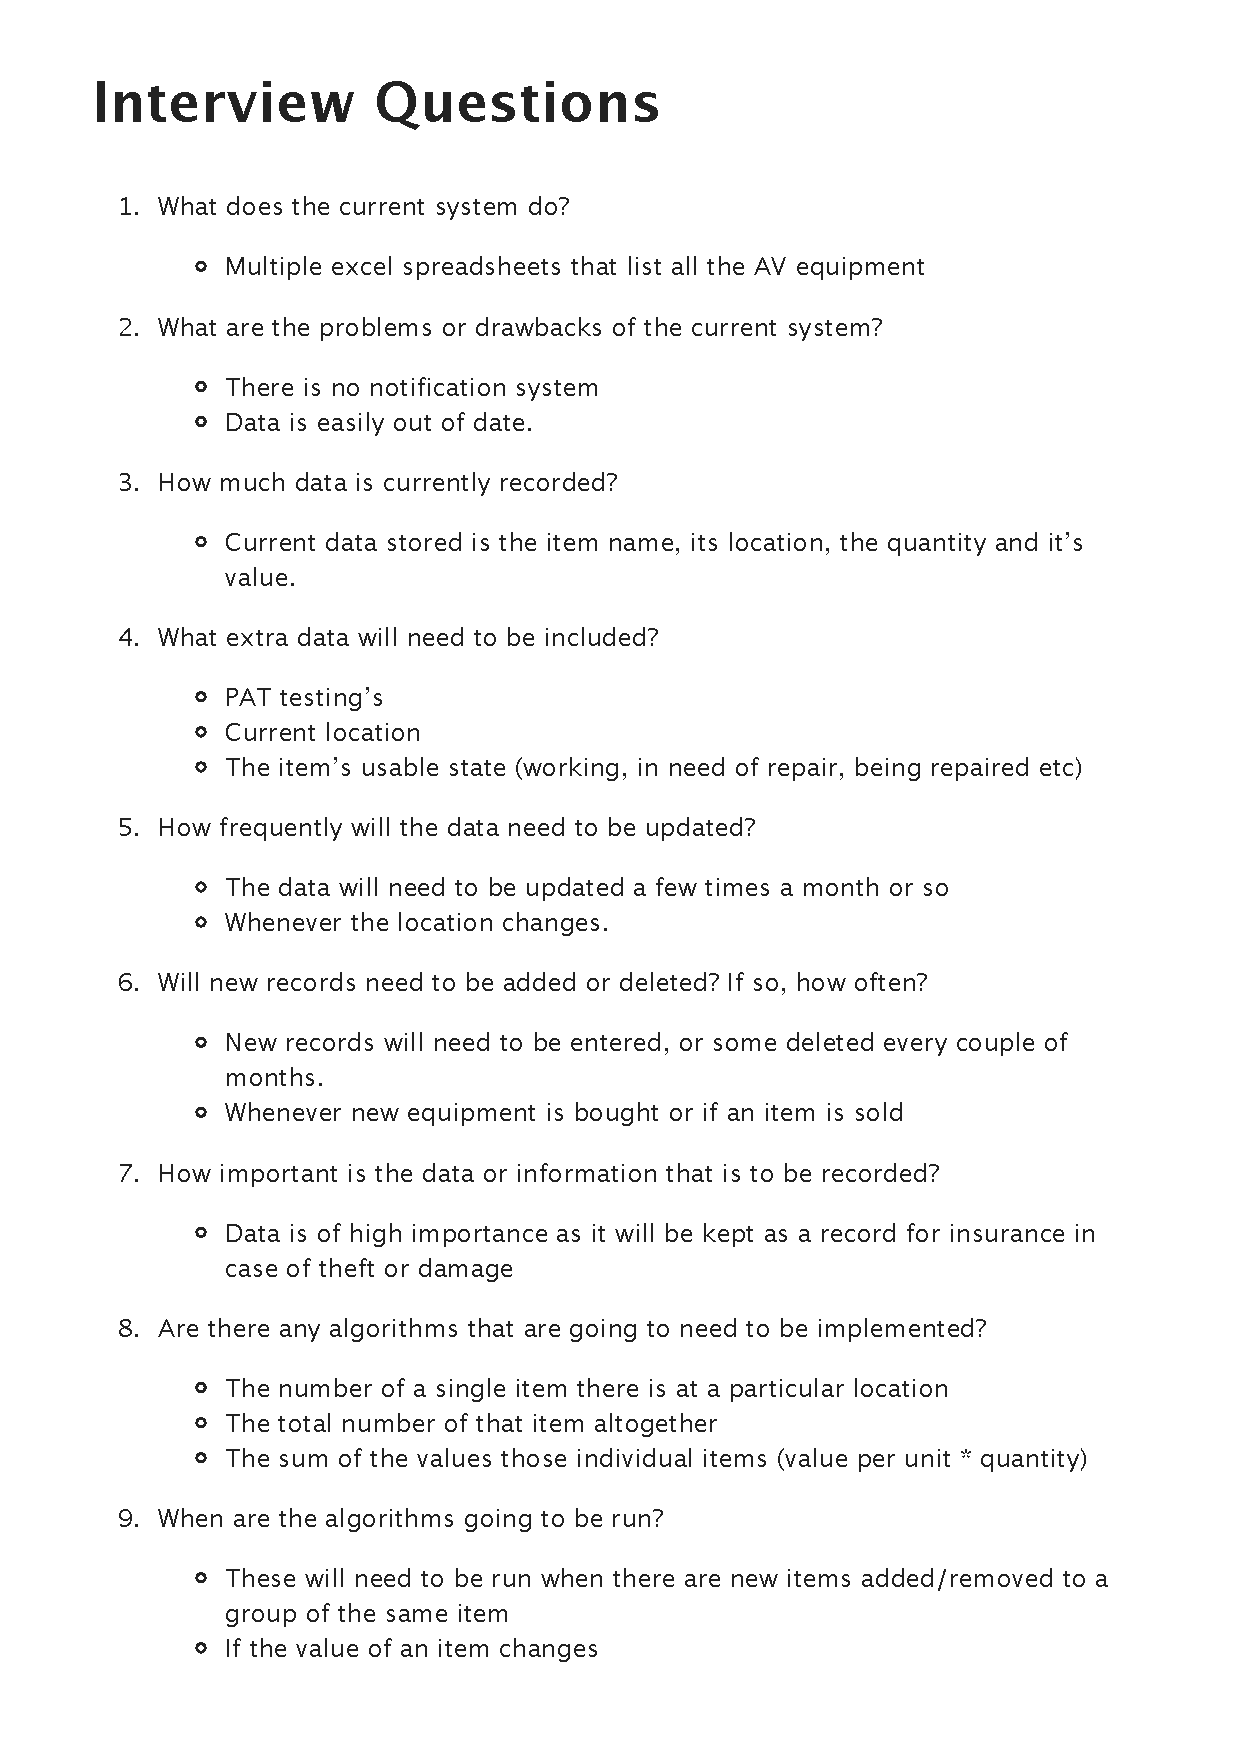
\includegraphics[page=1,width=\textwidth]{./Analysis/Interview/interview_questions.pdf}
\end{figure}		
		
\begin{figure}[H]		
    \caption{Interview Questions (pg 2)} \label{fig: Interview Questions}
    \includegraphics[page=2,width=\textwidth]{./Analysis/Interview/interview_questions.pdf}
\end{figure}		
		
\begin{figure}[H]		
    \caption{Interview Questions (pg 3)} \label{fig: Interview Questions}
    \includegraphics[page=3,width=\textwidth]{./Analysis/Interview/interview_questions.pdf}
\end{figure}

\subsection{The current system}

\subsubsection{Data sources and destinations}

In the current system, there are multiple data sources. The client and his colleagues as well as members of the AV crew for the church can enter data into the spreadsheet by using a computer in the office and accessing the on the server.

\subsubsection{Algorithms}

In the current system, there are only a few algorithms in place.
\bigskip

\begin{algorithm}[H]
    \caption{Algorithm 1, When new item is bought:}
\begin{algorithmic}[1]
\If{$Item = NewItem$}
    \SET{$Action$}{$Enter New Item$}
\ElsIf{$Item = ItemMatch$}
    \SET{$Action$}{$Update Item$}
\EndIf
\end{algorithmic}
\end{algorithm}

\begin{algorithm}[H]
    \caption{Algorithm 2, When an item is sold or replaced:}
\begin{algorithmic}[1]
\If{$Item = Sold$}
    \SET{$Action$}{$Update Quantity$}
\ElsIf{$Item = Damaged$}
    \SET{$Action$}{$Update Quantity$}
    \SET{$Action$}{$File Insurance Claim$}
\ElsIf{$Item = Stolen$}
    \SET{$Action$}{$File Insurance Claim$}
\EndIf
\end{algorithmic}
\end{algorithm}

\subsubsection{Data flow diagrams}

\begin{center}
    \begin{figure}[H]
        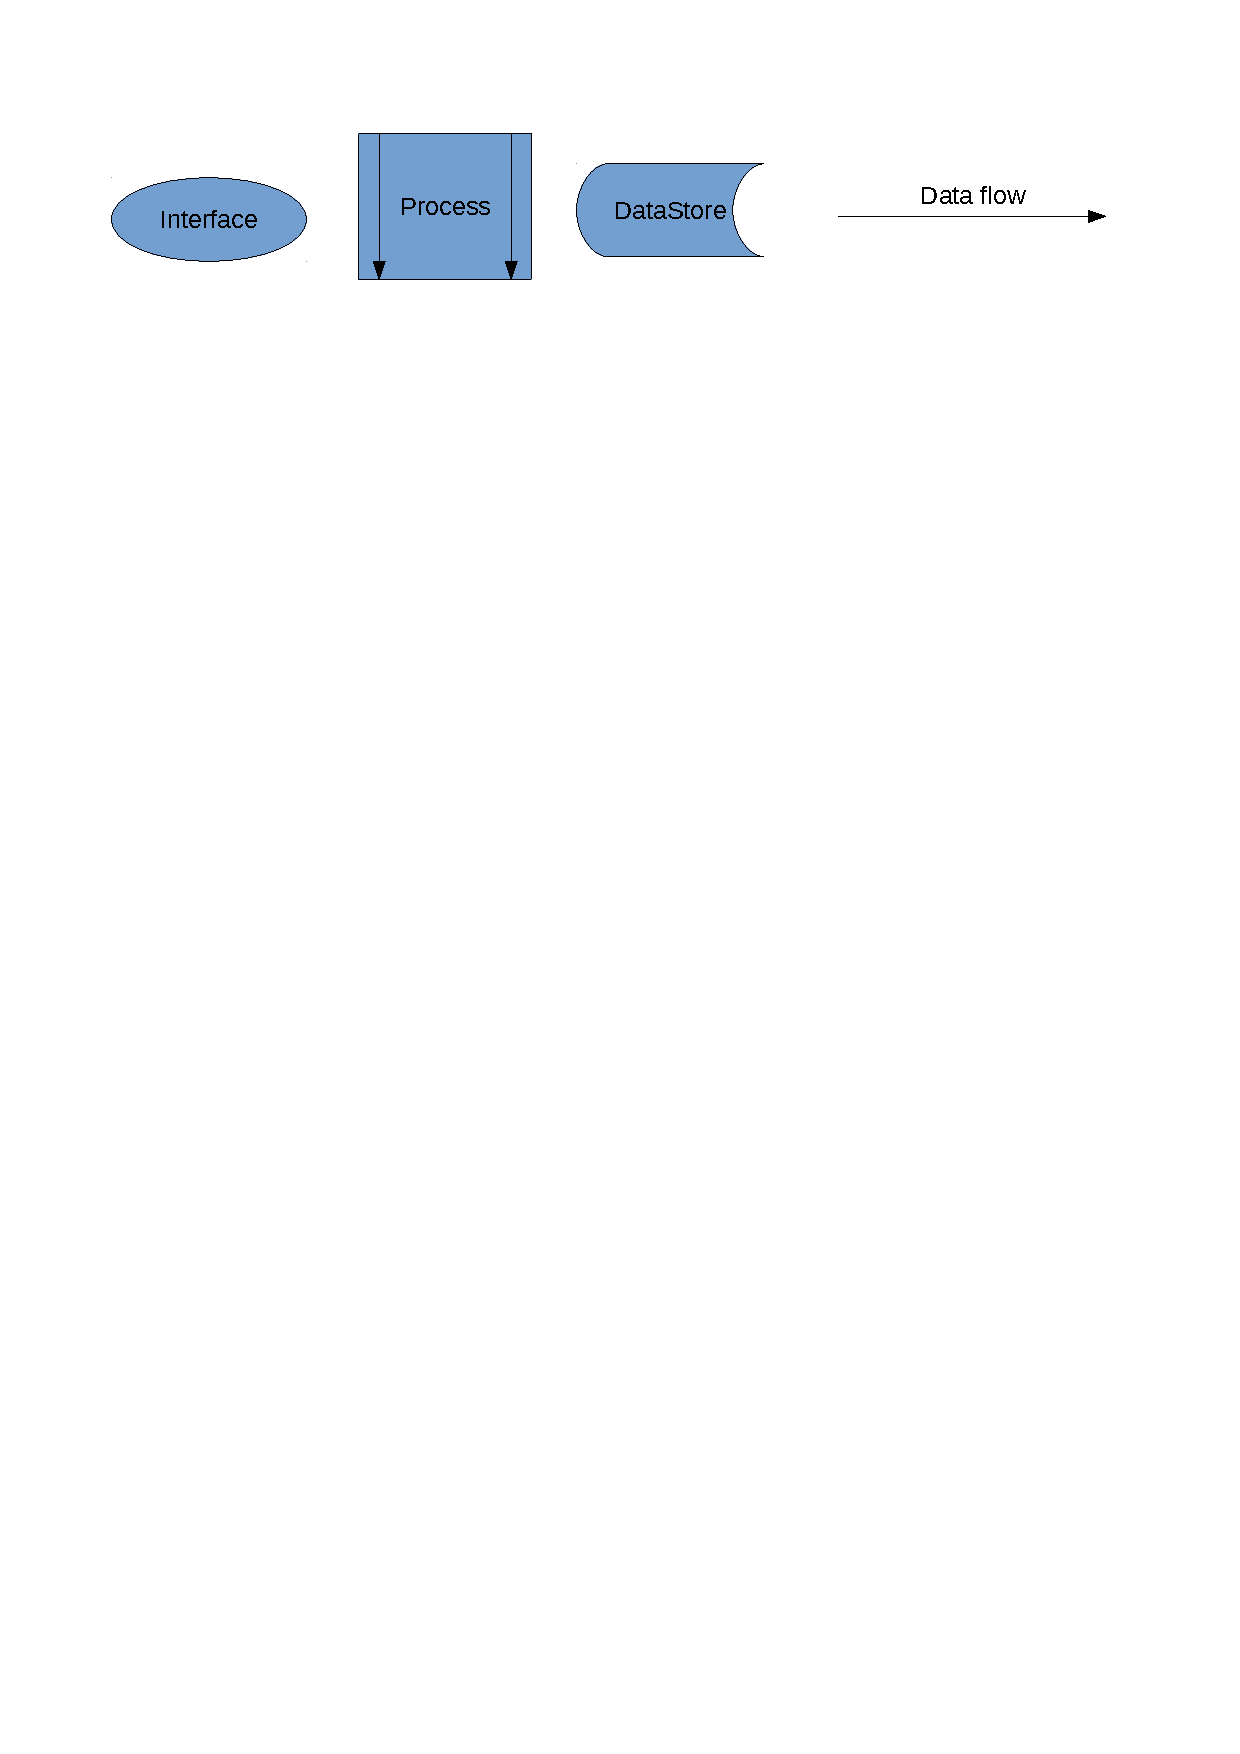
\includegraphics[width=\textwidth]{./Analysis/Dataflow/DFD_analysis_key.pdf}
        \caption{Flow Diagram Key.} \label{fig:print_function_result}
    \end{figure}

    \begin{figure}[H]
        \centerline{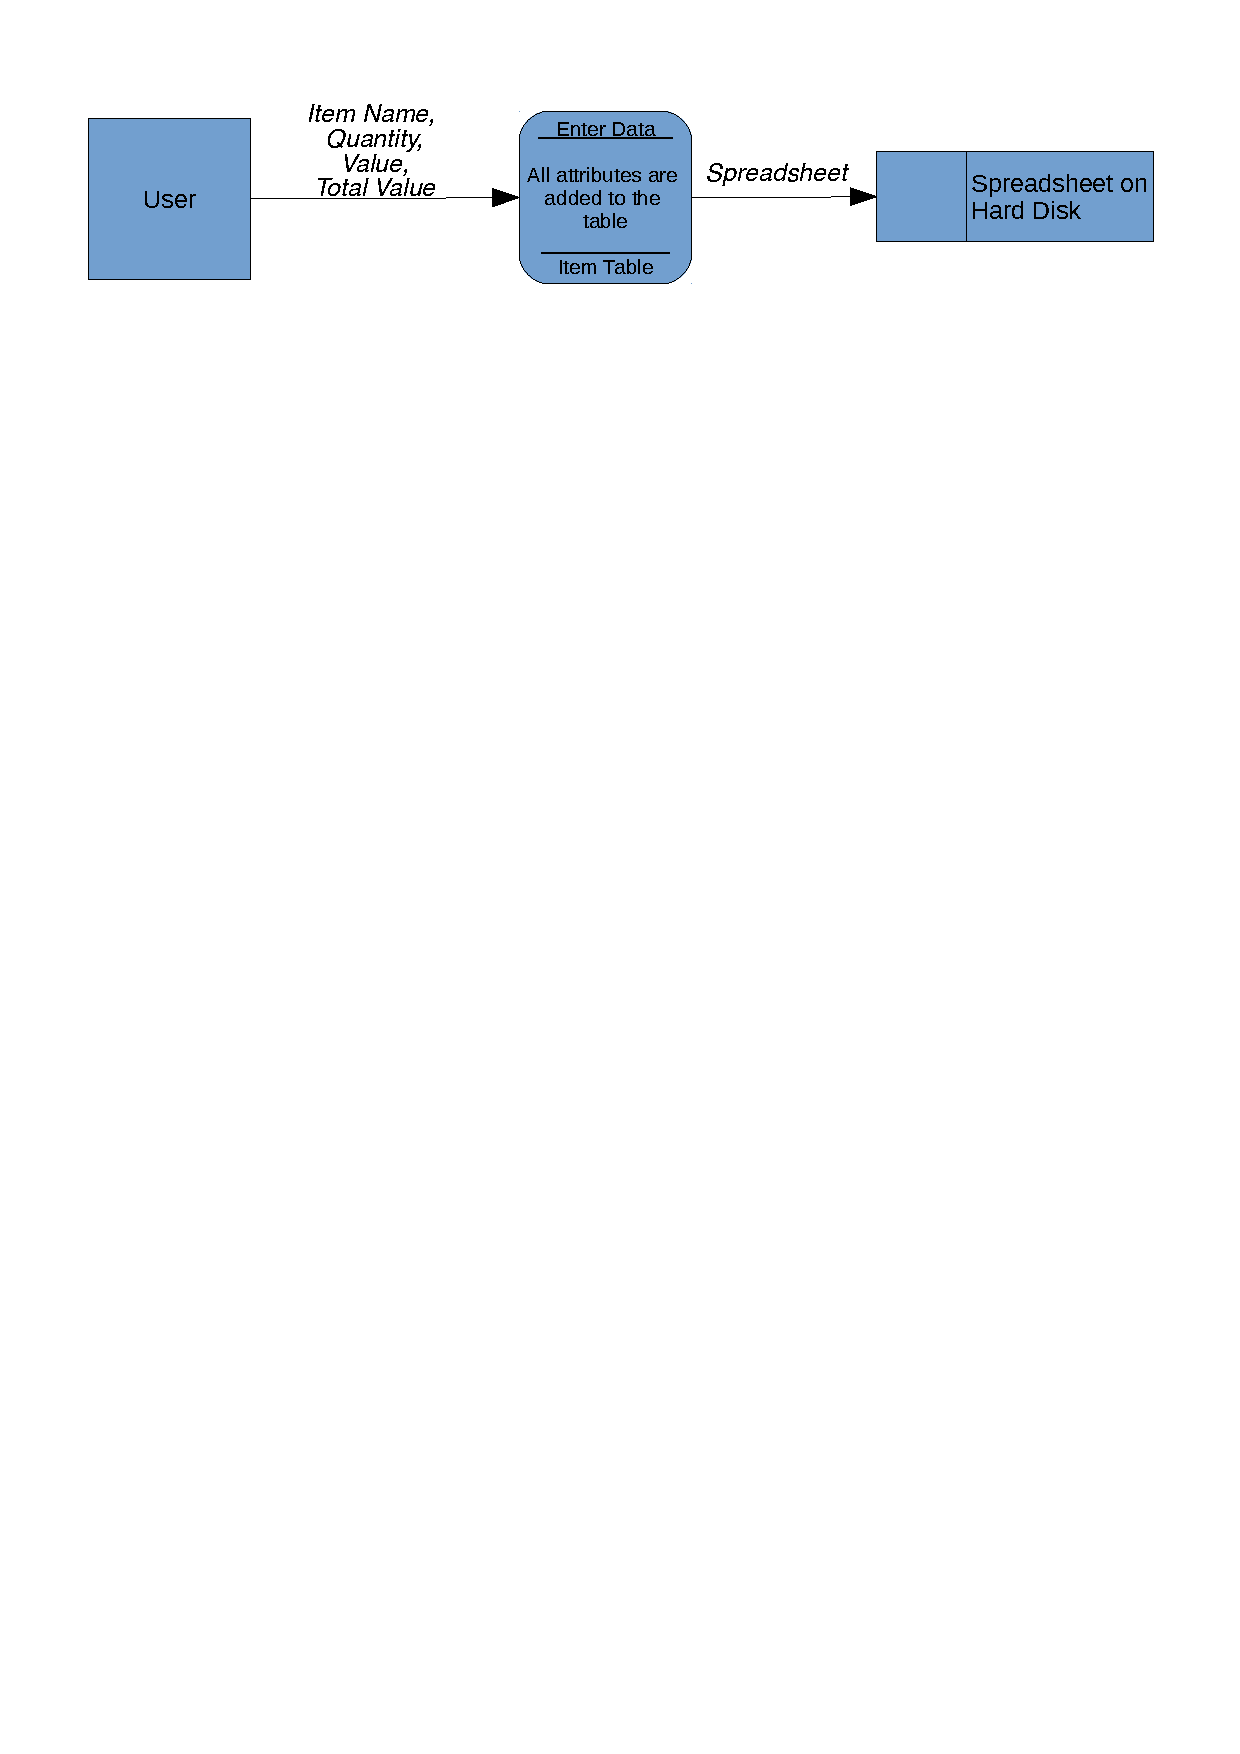
\includegraphics[width=\textwidth]{./Analysis/Dataflow/Old_System/Old_Sys_DFD_analysis_new_item.pdf}}
        \caption{Entering a new item.} \label{fig:print_function_result}
    \end{figure}

    \begin{figure}[H]
        \centerline{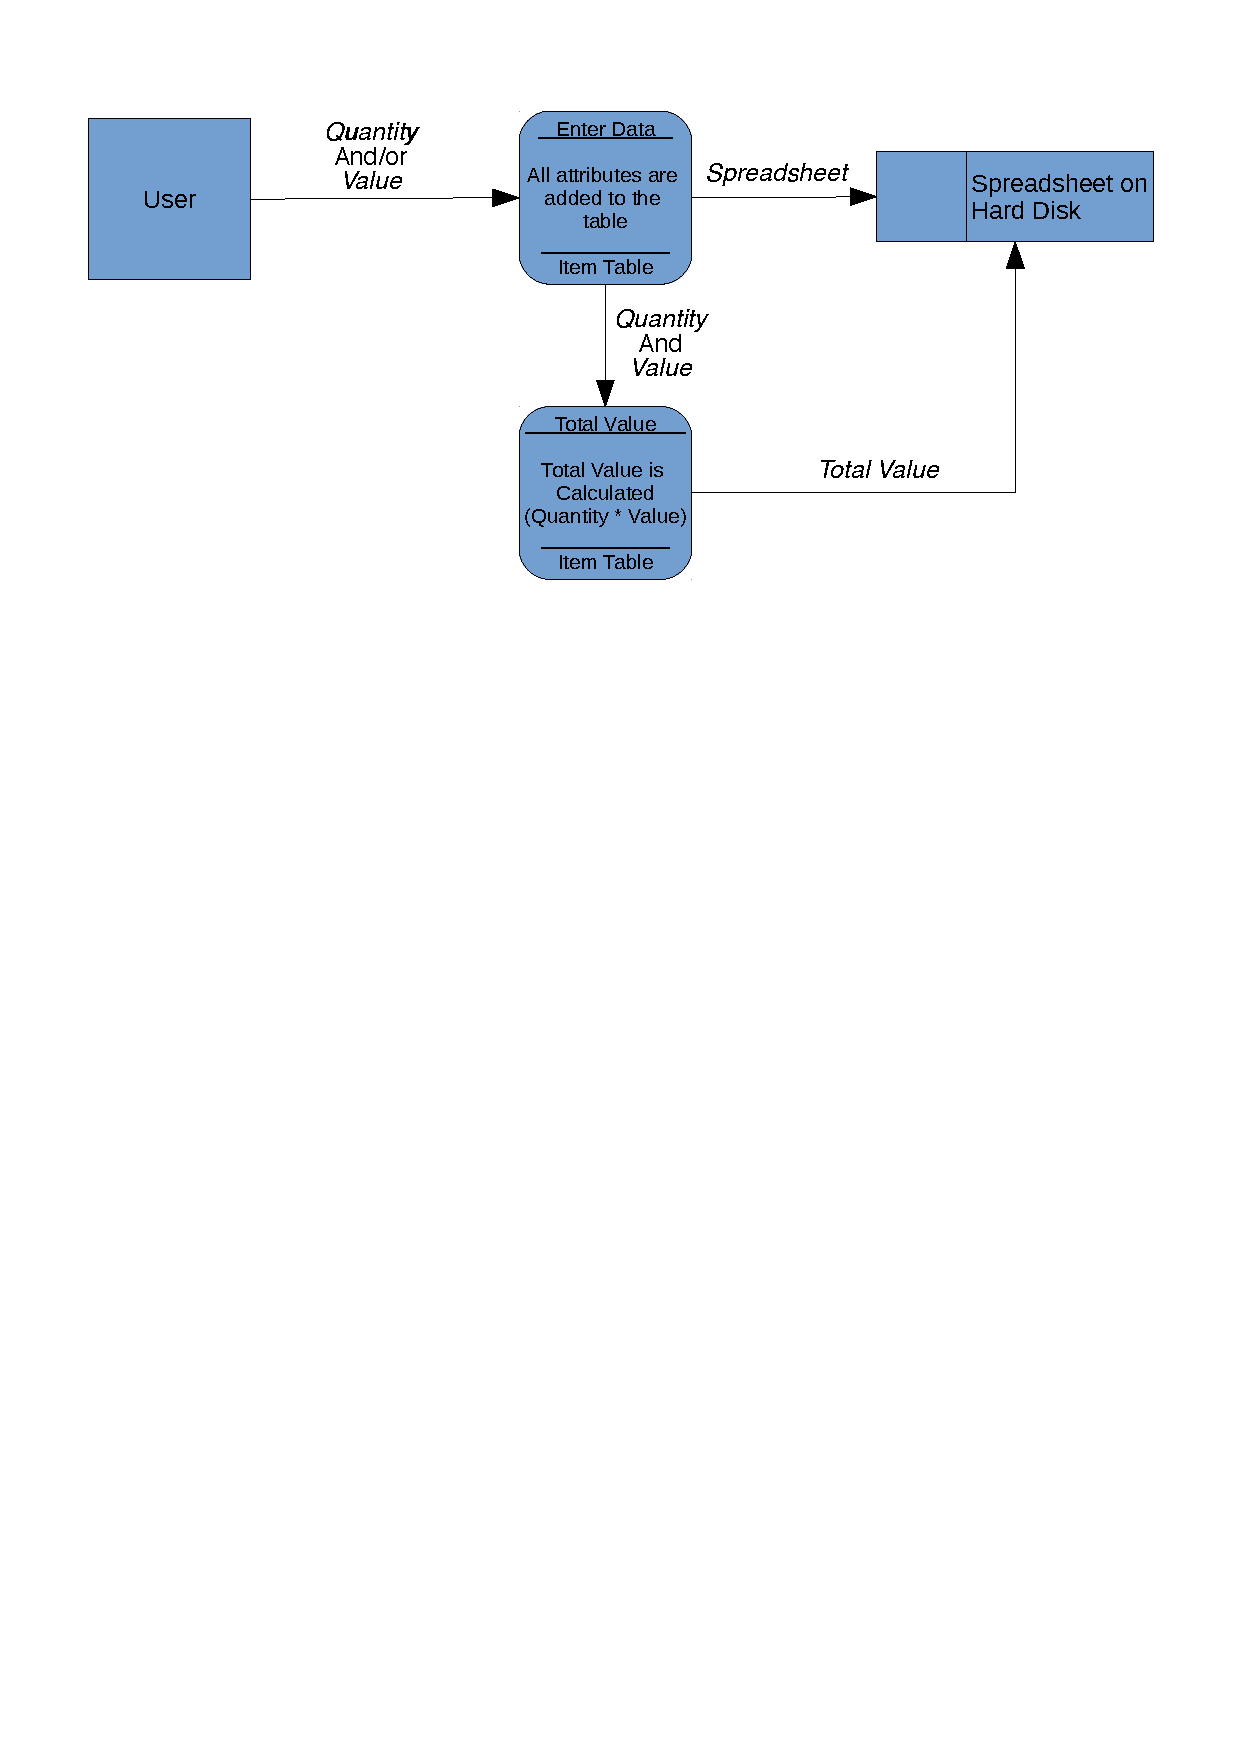
\includegraphics[width=\textwidth]{./Analysis/Dataflow/Old_System/Old_Sys_Data_flow_update.pdf}}
        \caption{Updating an item that already exists in the table.} \label{fig:print_function_result}
    \end{figure}
    
    \begin{figure}[H]
        \centerline{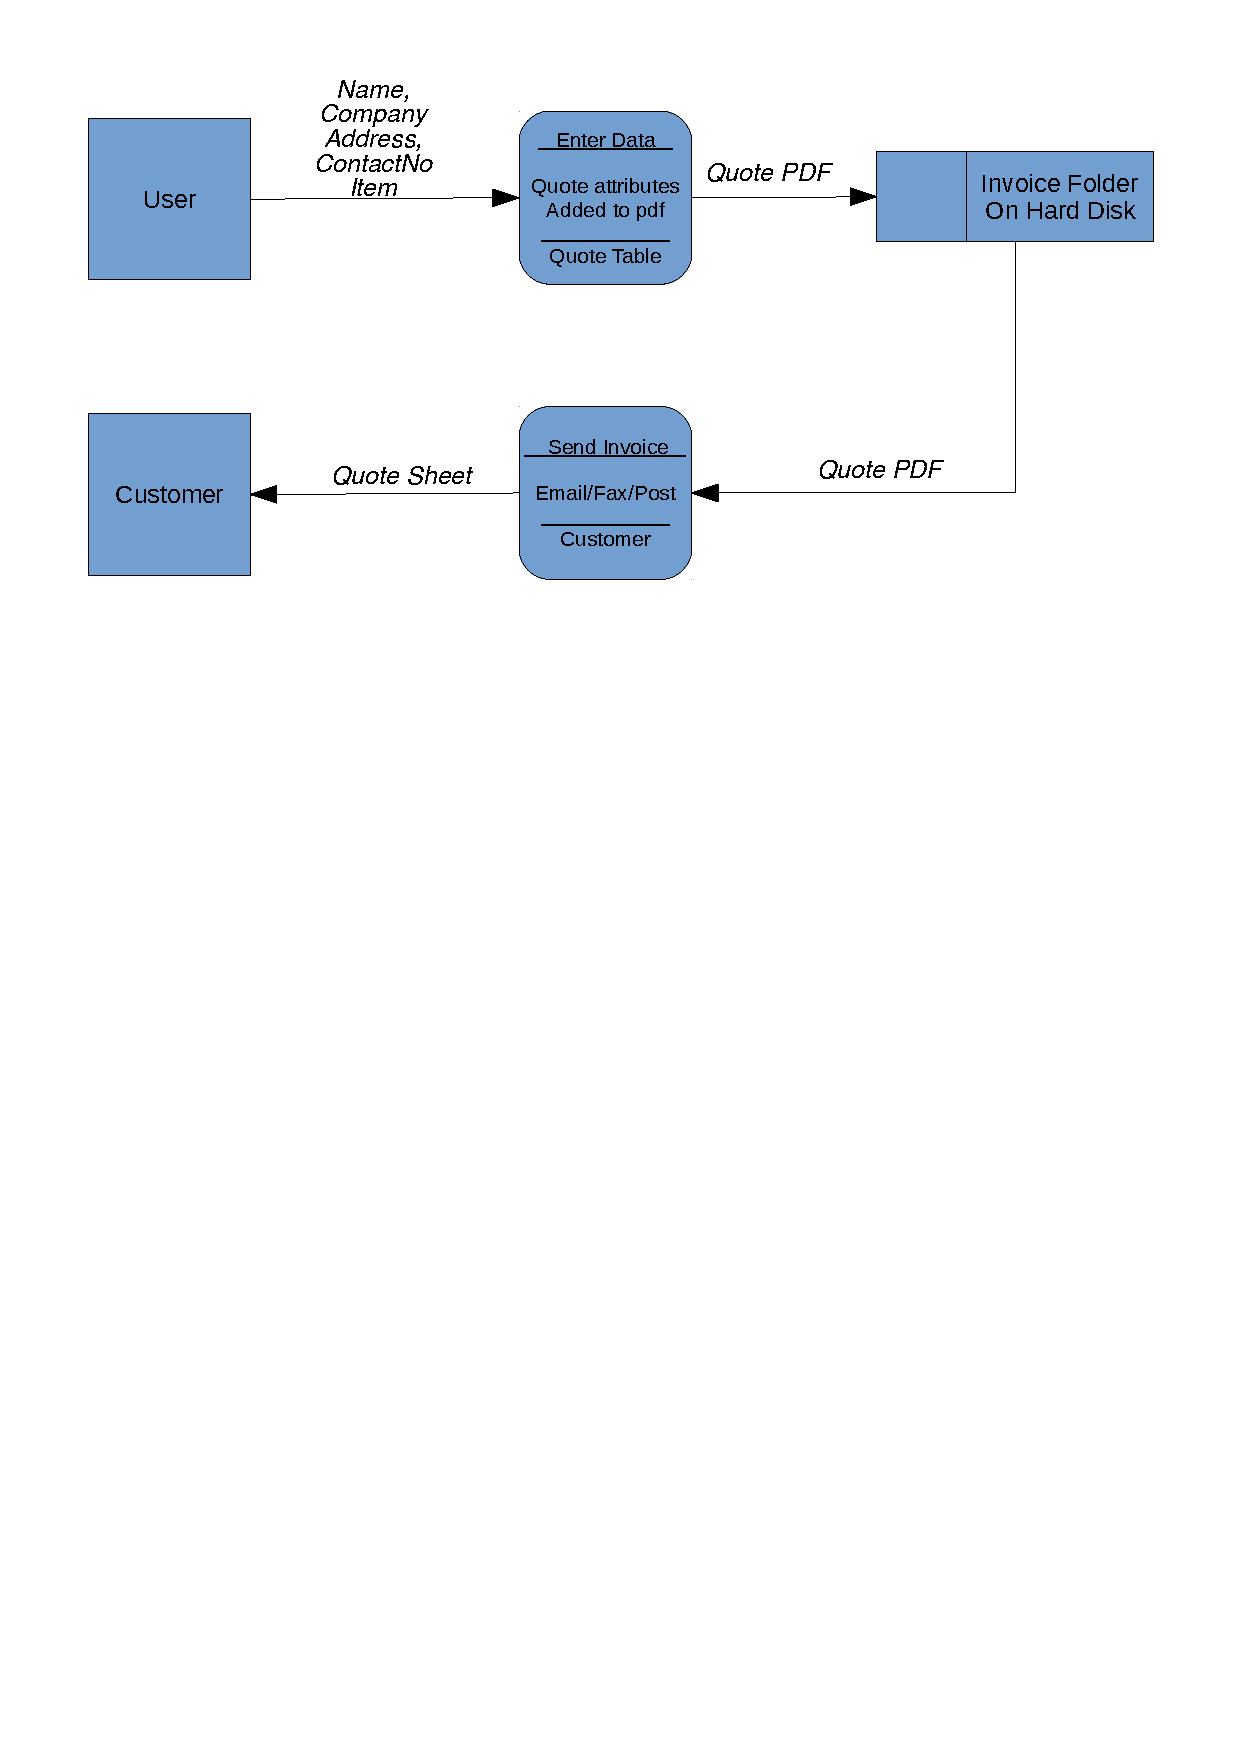
\includegraphics[width=\textwidth]{./Analysis/Dataflow/Old_System/Old_Sys_Data_flow_quote.pdf}}
        \caption{Creating and sending the initial quote for a loan.} \label{fig:print_function_result}
    \end{figure}
    
    \begin{figure}[H]
        \centerline{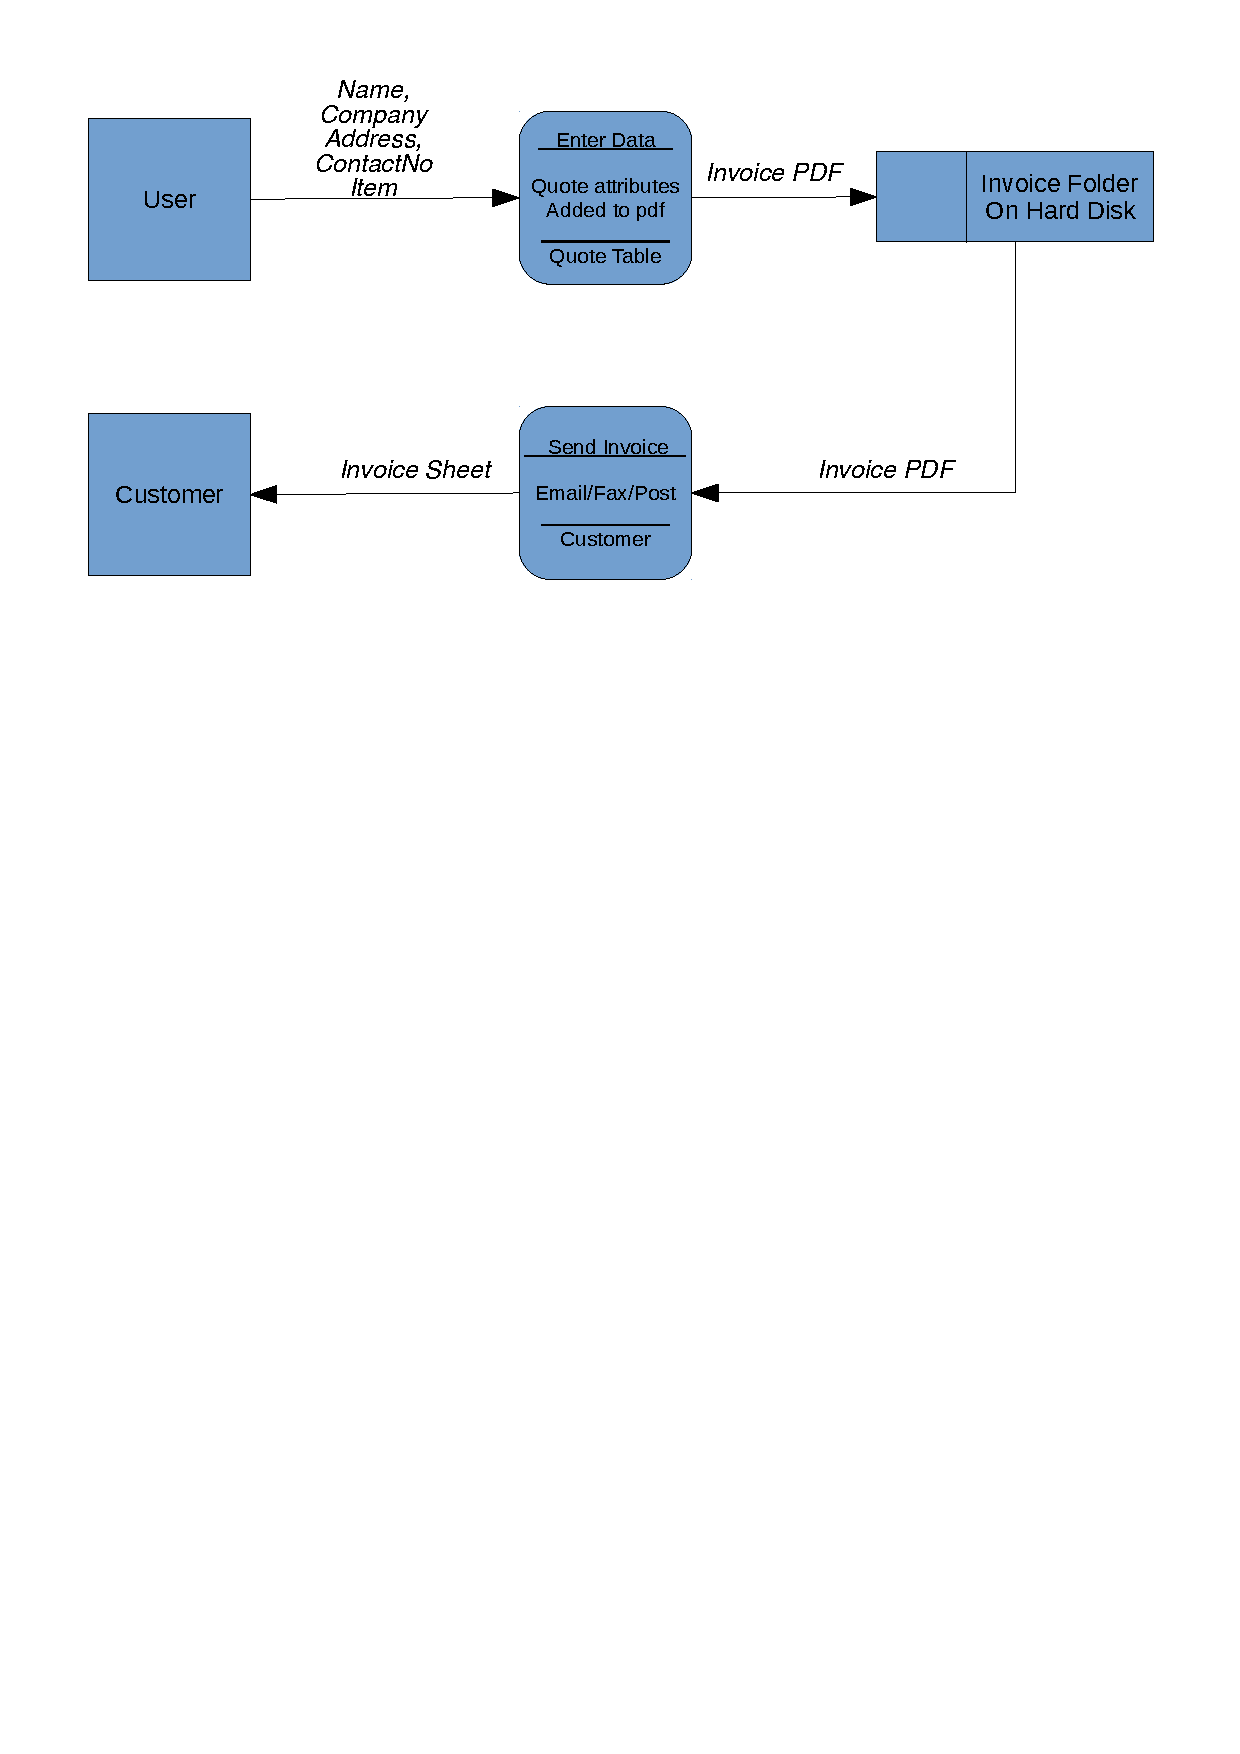
\includegraphics[width=\textwidth]{./Analysis/Dataflow/Old_System/Old_Sys_Data_flow_invoice.pdf}}
        \caption{Creating and sending the final invoice for a loan.} \label{fig:print_function_result}
    \end{figure}
\end{center}

\newpage

\subsubsection{Input Forms, Output Forms, Report Formats}

Josh has provided me with a screenshot of him entering some data into his current system. I have boxed out confidential information such as item values and their respective sub-total values:\\

\begin{figure}[H]
    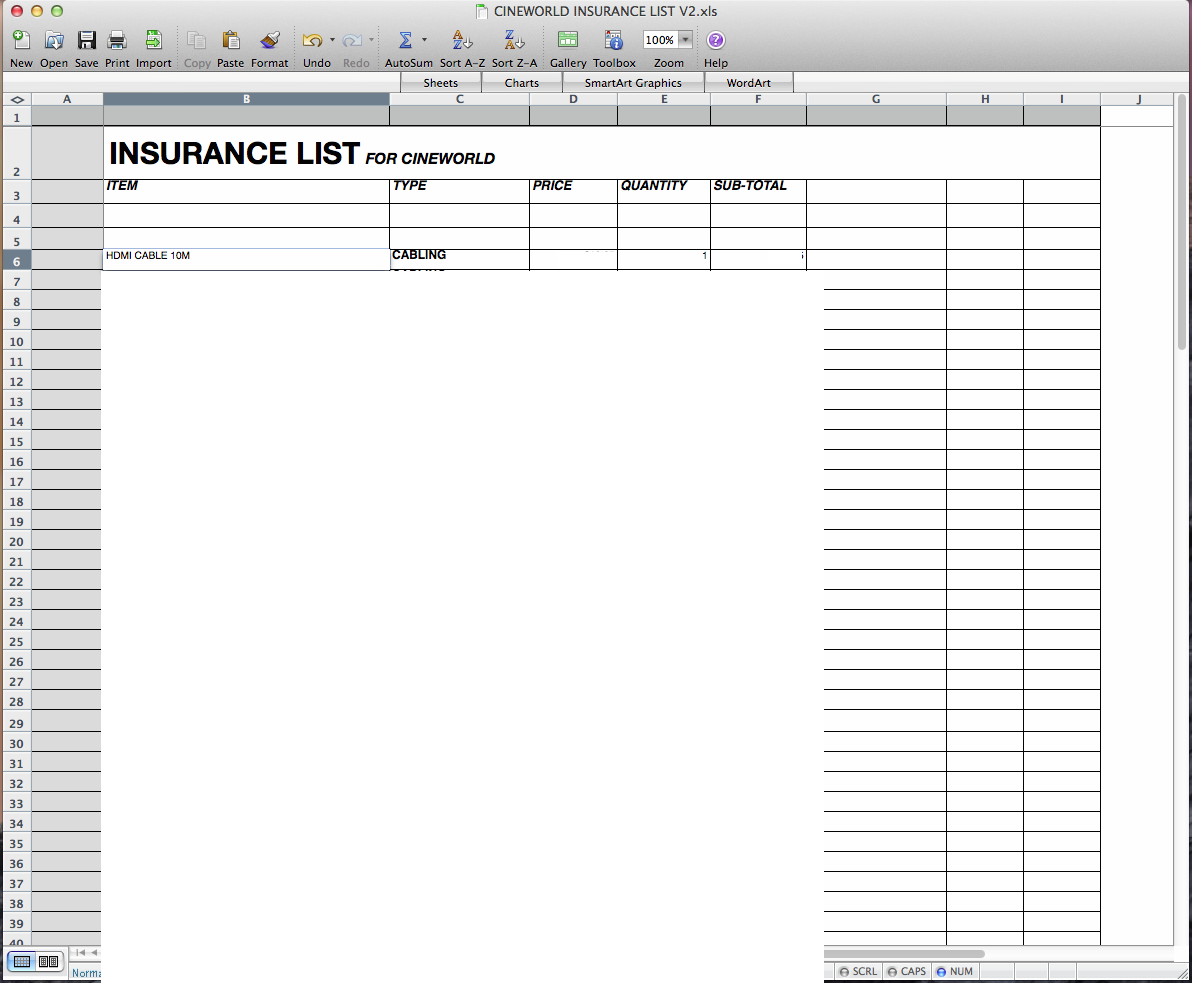
\includegraphics[width=\textwidth]{./Analysis/Forms/enter_data.png}
    \caption{Josh Entering Item Name.} \label{fig:print_function_result}
\end{figure}

\newpage

\noindent Here is an screen shot showing the calculation used to get the Sub-Total Value:

\begin{figure}[H]
    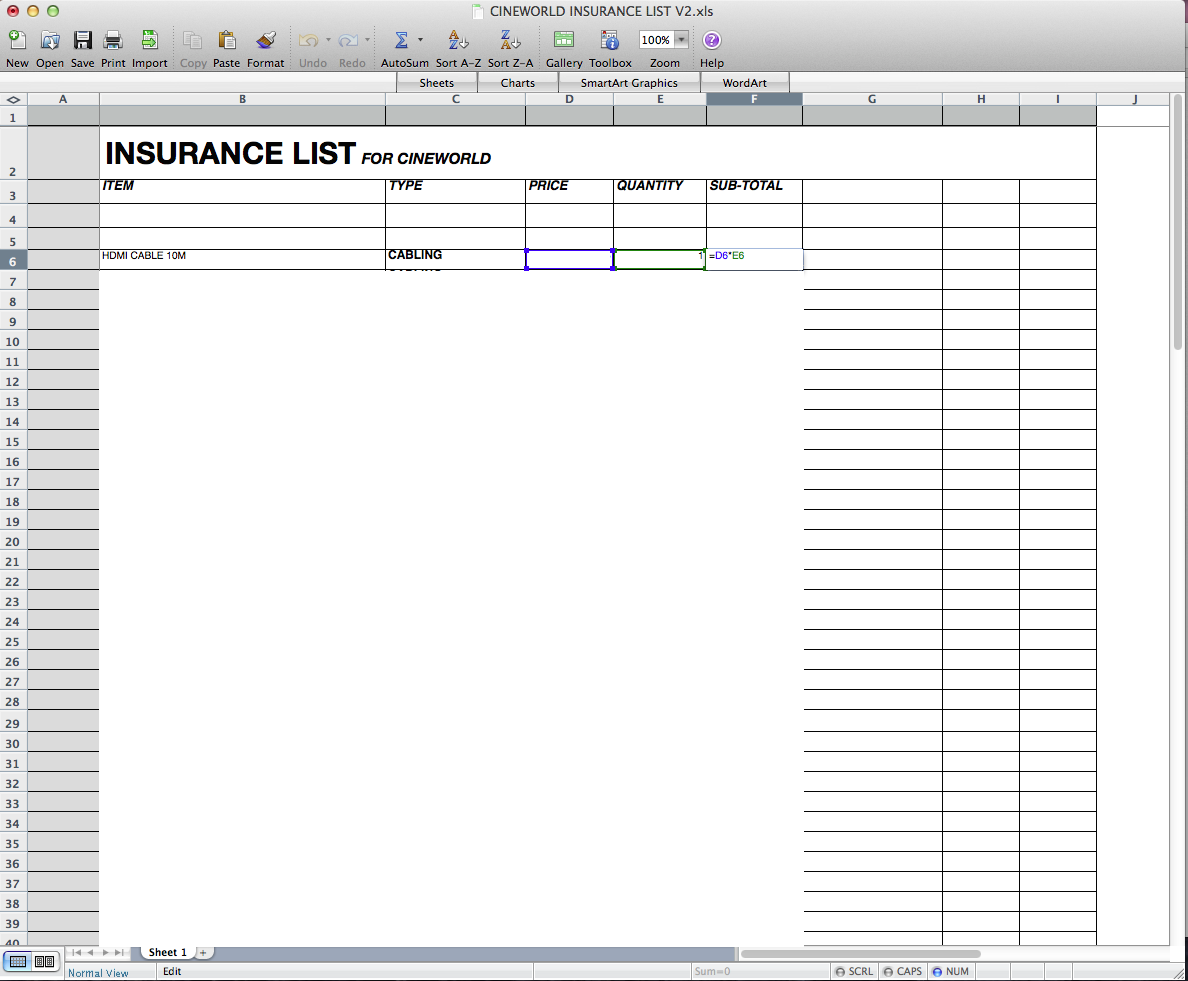
\includegraphics[width=\textwidth]{./Analysis/Forms/sub_total_calc.png}
    \caption{Sub-Total Calculation.} \label{fig:print_function_result}
\end{figure}

\subsection{The proposed system}

\subsubsection{Data sources and destinations}

The Following table shows the proposed data and their respective sources and destinations.

\begin{center}
        \begin{tabular}{|p{2cm}|p{3cm}|p{3cm}|p{3cm}|}
            \hline
            \textbf{Source} & \textbf{Data} & \textbf{Data Type} & \textbf{Destination} \\ \hline
            Generated & \textbf{ItemTypeID} & Integer & Database - ItemType Table \\ \hline
            User & ItemType & Text & Database - ItemType Table \\ \hline
            - & - & - & - \\ \hline
            Generated & \textbf{LocationID} & Integer & Database - Location Table \\ \hline
            User & Location & Text & Database - Location Table \\ \hline
            - & - & - & - \\ \hline
            Generated & \textbf{ItemID} & Integer & Database - Item Records \\ \hline
            Database - ItemType Table & \emph{ItemTypeID} & Integer & Database - Item Table \\ \hline
            Database - Location Table & \emph{LocationID} & Integer & Database - Item Table \\ \hline
            User & ItemName & Text & Database - Item Table \\ \hline
            User & Value & Real & Database - Item Table \\ \hline
            User & ItemQuantity & Integer & Database - Item Table \\ \hline
            User & SubTotal & Real & Database - Item Table \\ \hline
            User & OnLoan & Boolean & Database - Item Table \\ \hline
            \end{tabular}
\end{center}

\begin{center}
        \begin{tabular}{|p{2cm}|p{3cm}|p{3cm}|p{3cm}|}
            \hline
            \textbf{Source} & \textbf{Data} & \textbf{Data Type} & \textbf{Destination} \\ \hline
            Generated & \textbf{LoanListingID} & Integer & Database - LoanListing Table \\ \hline
            Database - Item Table & \emph{ItemID} & Integer & Database - LoanListing Table \\ \hline
            User & LoanQuantity & Integer & Database - LoanListing Table \\ \hline
            - & - & - & - \\ \hline
            Generated & \textbf{CustomerLoanID} & Integer & Database - Loan Table \\ \hline
            Database - Customer Table & \emph{CustomerID} & Integer & Database - Loan Table \\ \hline
            User & LoanRate & Real & Database - Loan Table \\ \hline
            User & LoanLength(Days) & Integer & Database - Loan Table \\ \hline
            Calculated & LoanCost & Real & Database - Loan Table \\ \hline
            - & - & - & - \\ \hline
            Generated & \textbf{CustomerID} & Integer & Database - Customer Table \\ \hline
            User & Forename & Text & Database - Customer Table \\ \hline
            User & Lastname & Text & Database - Customer Table \\ \hline
            User & Company & Text & Database - Customer Table \\ \hline
            User & Street & Text & Database - Customer Table \\ \hline
            User & Town & Text & Database - Customer Table \\ \hline
            User & County & Text & Database - Customer Table \\ \hline
            User & PostCode & Text & Database - Customer Table \\ \hline
            User & MobileNumber & Text & Database - Customer Table \\ \hline
            User & LandLine & Text & Database - Customer Table \\ \hline
            User & Email & Text & Database - Customer Table \\ \hline
            \end{tabular}
\end{center}

\begin{center}
        \begin{tabular}{|p{2cm}|p{3cm}|p{3cm}|p{3cm}|}
            \hline
            \textbf{Source} & \textbf{Data} & \textbf{Data Type} & \textbf{Destination} \\ \hline
            Generated & \textbf{ItemTestID} & Integer & Database - ItemTest Table \\ \hline
            Database - PATtest Records & \emph{PATtestID} & Integer & Database - ItemTest Table \\ \hline
            User & ItemDescription & Text & Database - ItemTest Table \\ \hline
            User & ItemClass & Integer & Database - ItemTest Table \\ \hline
            User & FuseRating & Text & Database - ItemTest Table \\ \hline
            User & TestUsed & Text & Database - ItemTest Table \\ \hline 
            User & ProtectiveCondTest & Integer & Database - ItemTest Table \\ \hline
            User & InsulationTest & Text & Database - ItemTest Table \\ \hline
            User & Leakage & Float & Database - ItemTest Table \\ \hline
            User & TestResult & Boolean & Database - ItemTest Table \\ \hline
            - & - & - & - \\ \hline
            Generated & \textbf{PATtestID} & Integer & Database - PATtest Table \\ \hline
            User & TestDate & Date & Database - PATtest Table \\ \hline
        \end{tabular}
\end{center}


\subsubsection{Data flow diagram}

\begin{figure}[H]
    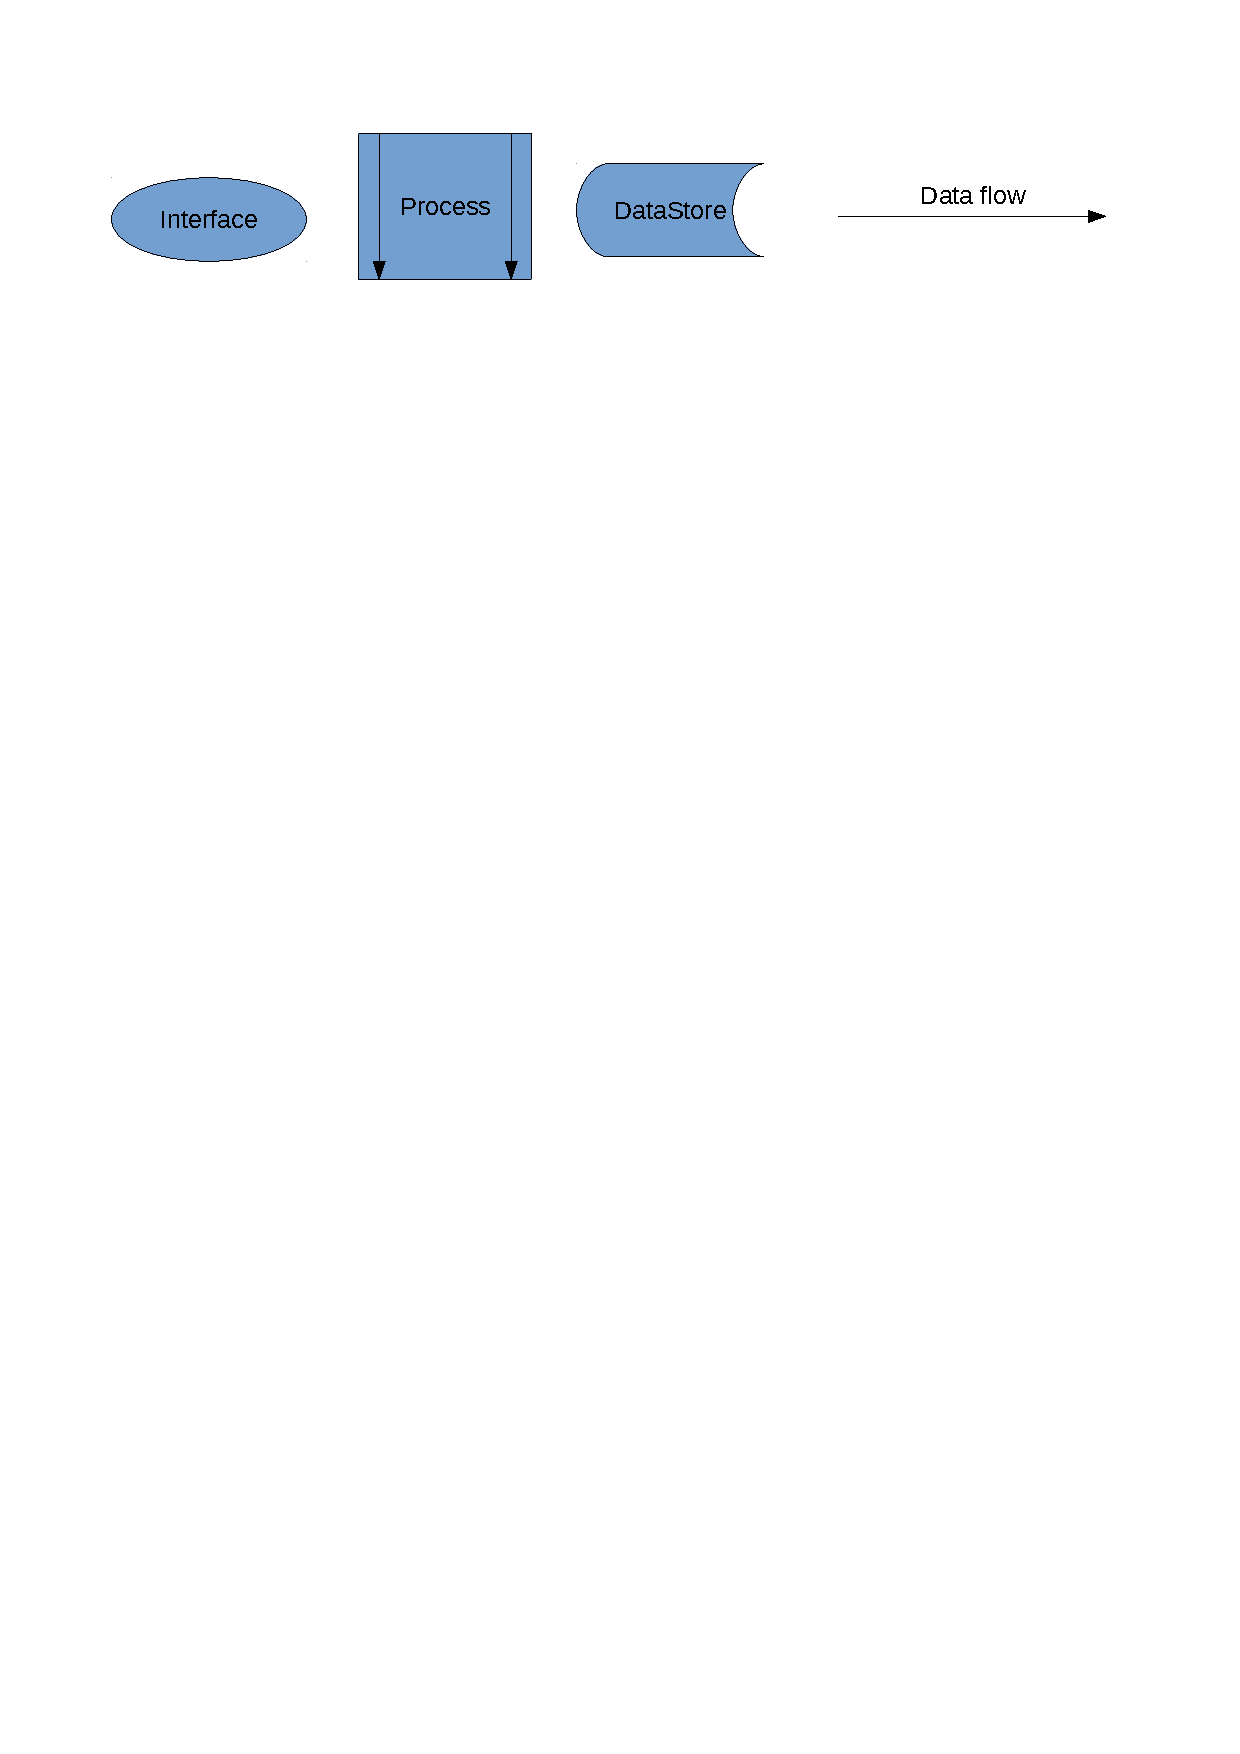
\includegraphics[width=\textwidth]{./Analysis/Dataflow/DFD_analysis_key.pdf}
    \caption{Flow Diagram Key.} \label{fig:print_function_result}
\end{figure}

\begin{figure}[H]
    \caption{Enter New Item.} \label{fig:print_function_result}
    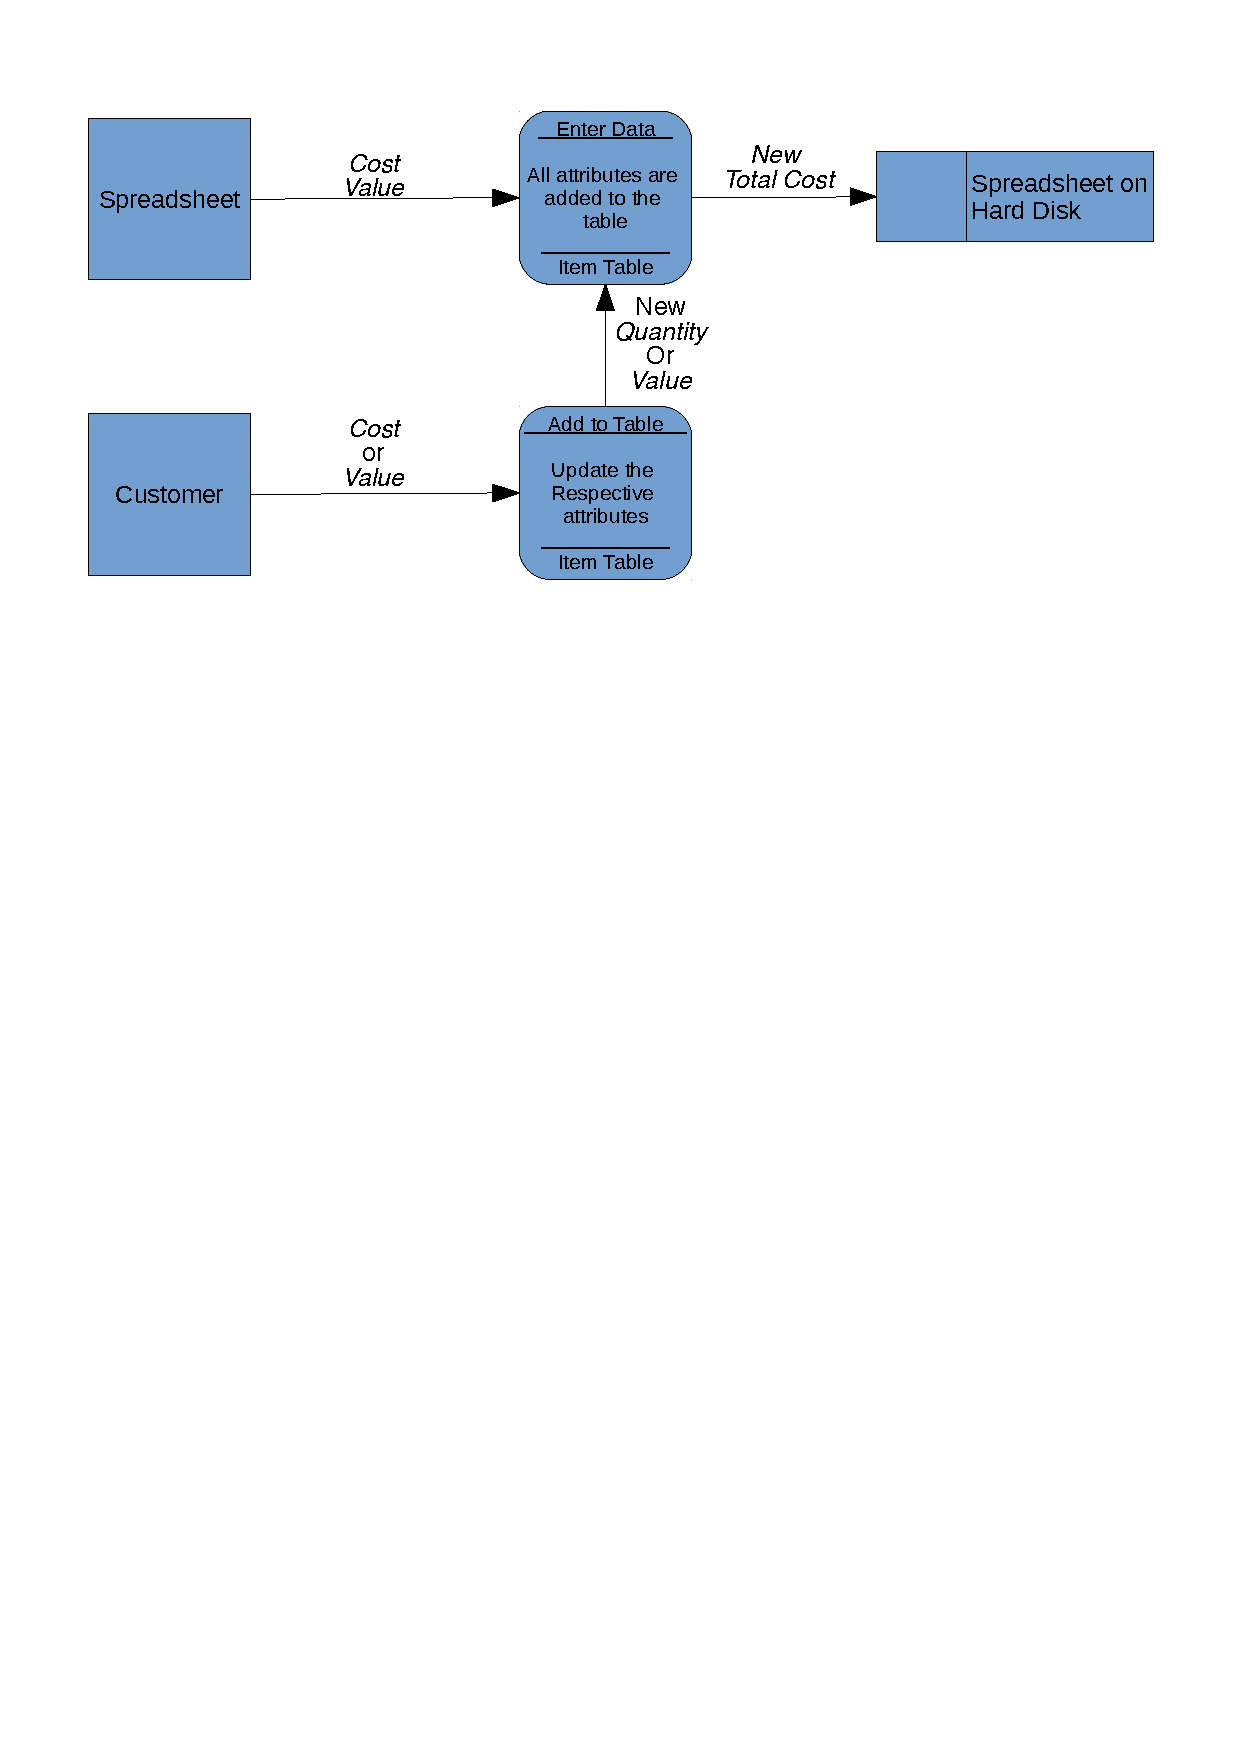
\includegraphics[width=\textwidth]{./Analysis/Dataflow/New_System/Data_flow_new.pdf}
\end{figure}

\begin{figure}[H]
    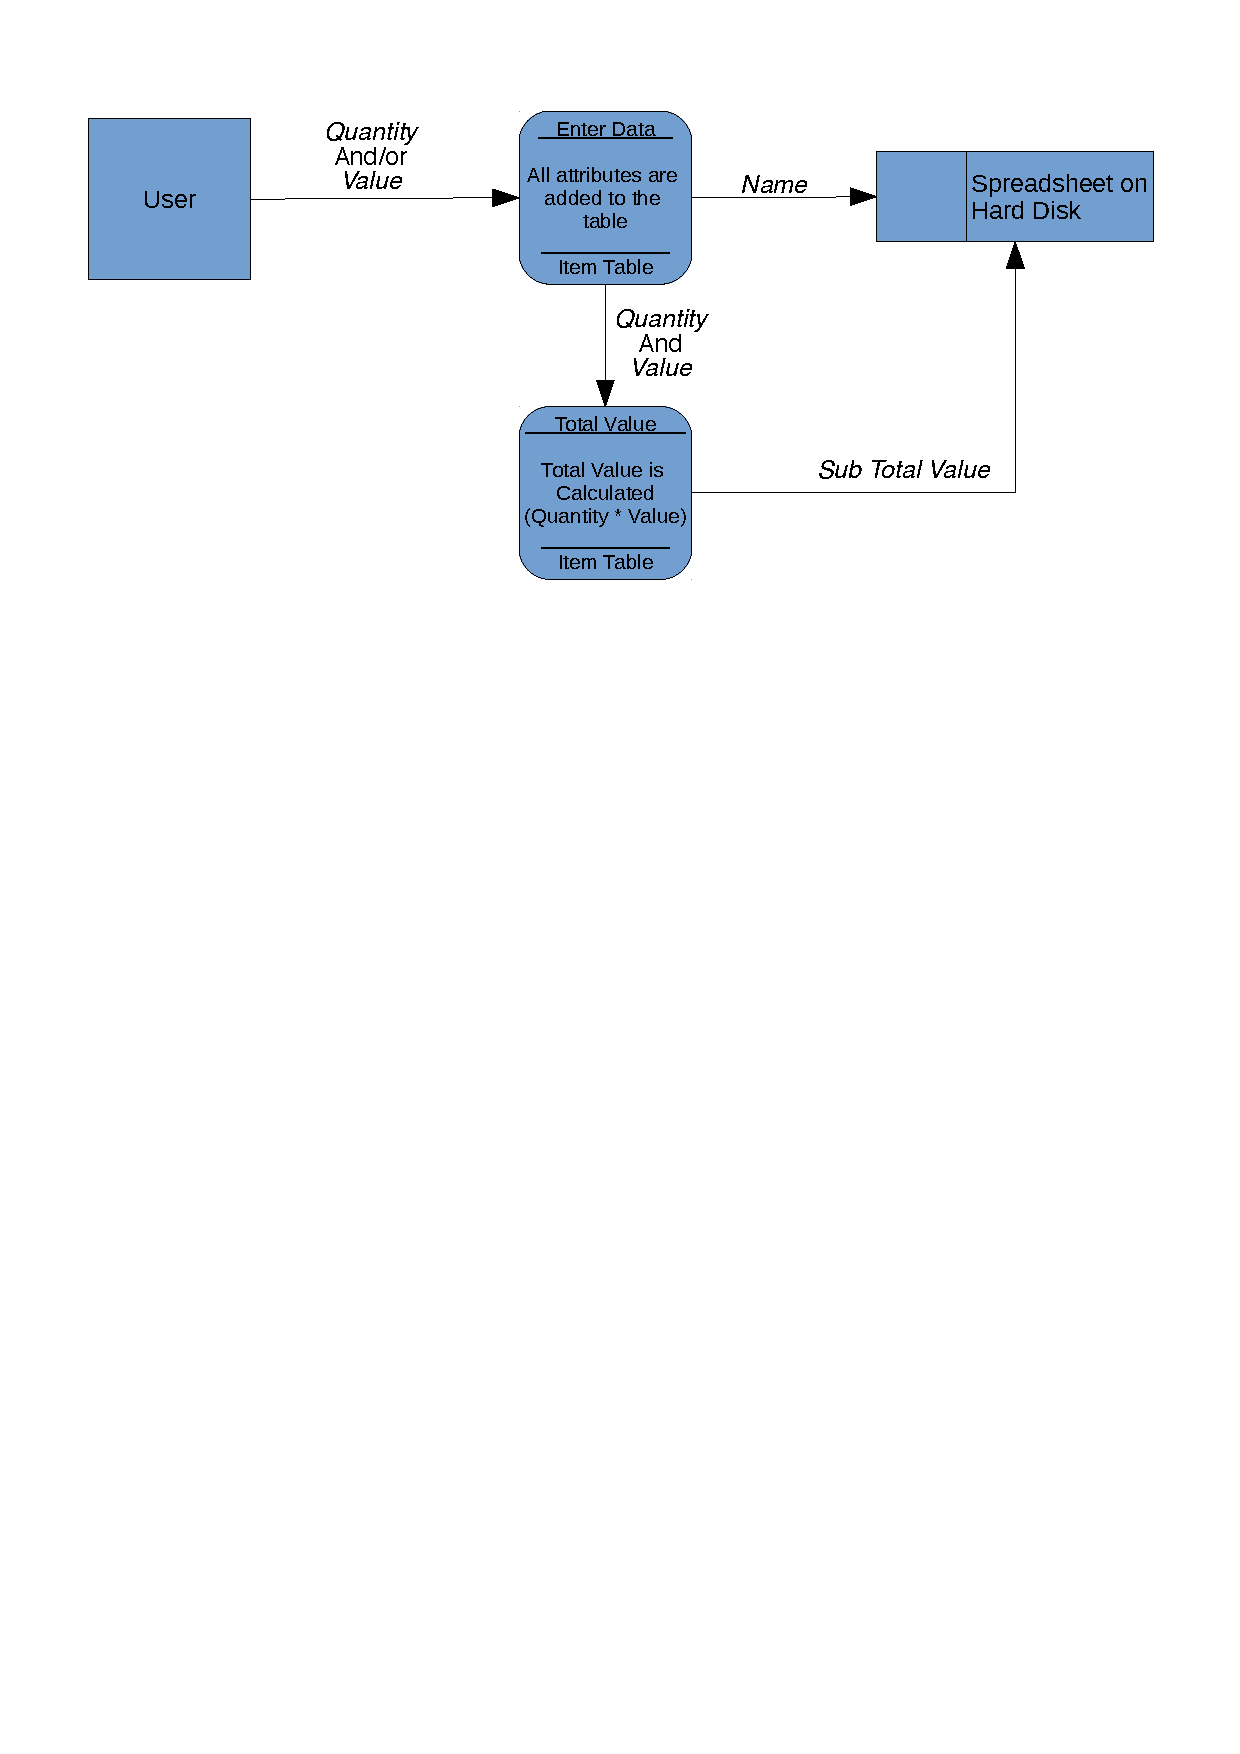
\includegraphics[width=\textwidth]{./Analysis/Dataflow/New_System/Data_flow_update.pdf}
    \caption{Enter New Item.} \label{fig:print_function_result}
\end{figure}



\subsubsection{Data dictionary}

\begin{landscape}

    \begin{center}
    \subsubsection{Data dictionary}
    \end{center}
    
    \begin{center}
        \begin{tabular}{|p{3cm}|p{2cm}|p{3cm}|p{2cm}|p{2cm}|p{5cm}|}
            \hline
            \textbf{Name} & \textbf{Data Type} & \textbf{Length} & \textbf{Validation} & \textbf{Example Data} & \textbf{Comment} \\ \hline
            ItemTypeID & Integer & 1-435 & Range & 253 & This is the \textbf{Primary Key} for the ItemType class, and foreign key for the Item class \\ \hline
            ItemType & Text & 5-40 Characters & Length & Arkaos Server & This holds the description of each type of Item. \\ \hline
            LocationID & Integer & 1-3 Figures & Range & 1,300 & This is the \textbf{Primary Key} for the Location class and a \emph{Foreign Key} for the Item class \\ \hline
            Location & Text & 1-30 Characters & Length & Main Offices  & This holds the name of the locations \\ \hline
            \end{tabular}
    \end{center}
\end{landscape}


\begin{landscape}
    \begin{center}
        \begin{tabular}{|p{3cm}|p{2cm}|p{3cm}|p{2cm}|p{2cm}|p{5cm}|}
            \hline
            \textbf{Name} & \textbf{Data Type} & \textbf{Length} & \textbf{Validation} & \textbf{Example Data} & \textbf{Comment} \\ \hline
            ItemID & Integer & 1-435 & Range & 253 & This is the \textbf{Primary Key} for the Item class, and foreign key for the Loan and PATtest classes \\ \hline
            ItemName & Text & 5-40 Characters & Length & Arkaos Server & This gives the name of each item entered \\ \hline
            Value & Real & 2-5 Figures & Range & 1,300 & This holds the data for the monetary value for each item \\ \hline
            ItemQuantity & Integer & 0-100 & Range & 35 & This holds the data for the number of each item owned \\ \hline
            SubTotal & Real & 2-8 Figures & Range & 250 & This  is calculated for each item by multiplying the value by the quantity \\ \hline
            OnLoan & Boolean & True/False & Status Check & True & This holds the data of whether an item is on loan or not. Will be displayed as "Yes" or "No" \\ \hline
            \end{tabular}
    \end{center}
\end{landscape}


\begin{landscape}
    \begin{center}
        \begin{tabular}{|p{3cm}|p{2cm}|p{3cm}|p{2cm}|p{2cm}|p{5cm}|}
            \hline
            \textbf{Name} & \textbf{Data Type} & \textbf{Length} & \textbf{Validation} & \textbf{Example Data} & \textbf{Comment} \\ \hline
            LoanListingID & Integer & 1-435 & Range & 56 & This is the \textbf{Primary Key} for the LoanListing class \\ \hline
            ListingQuantity & Integer & 1-35 & Range & 4 & This holds the data for how many of an item has been loaned out \\ \hline
            CustomerLoanID & Integer & 1-435 & Range & 21 & This is the \textbf{Primary Key} for the Loan class \\ \hline
            LoanRate & Real & 1-5 Figures & Range & 75 & Holds data for how much is charged per day for the loan of an item \\ \hline
            LoanLength & Integer & 1-3 Figures & Range & 7 & Holds the data for the length of the loan \\ \hline
            LoanCost & Real & 1-4 Integers & Range & 250 & Holds the data for the amount to charge before the loan \\ \hline
        \end{tabular}
    \end{center}
\end{landscape}


\begin{landscape}
    \begin{center}
        \begin{tabular}{|p{2.3cm}|p{2cm}|p{3cm}|p{2cm}|p{4.6cm}|p{4cm}|}
            \hline
            \textbf{Name} & \textbf{Data Type} & \textbf{Length} & \textbf{Validation} & \textbf{Example Data} & \textbf{Comment} \\ \hline
            CustomerID & Integer & 1-255 & Range & 52 & This is the \textbf{Primary Key} for the Customer class \\ \hline
            Forename & Text & 3-20 Characters & Length & John & A field for the customers forename \\ \hline
            Lastname & Text & 3-20 Characters & Length & Smith & A field for the customers surname\\ \hline
            Company & Text & 3-20 Characters & Length & Digital Lighting Cambs & A field for the company's name\\ \hline
            Street & Text & 3-30 Characters & Length & 129 Cedar Crescent & A field for the company's Street address\\ \hline
            Town & Text & 3-30 Characters & Length & Sawston & A field for the company's Town \\ \hline
            County & Text & 3-20 Characters & Length & Cambs & A field for the company's County \\ \hline
            PostCode & Text & 6-7 Characters & Format & CB22 7RX & A field for the company's Postcode \\ \hline
            MobileNumber & Text & 11 Characters & Format & 07891234567 & A field for the customers mobile number\\ \hline
            LandLine & Text & 11 Characters & Format & 01234567890 & A field for the customers landline phone \\ \hline
            Email & Text & 7 - 30 Characters & Length & john.smith@example.com & A field for the customers email address\\ \hline
        \end{tabular}
    \end{center}
\end{landscape}


\begin{landscape}
    \begin{center}
        \begin{tabular}{|p{3.4cm}|p{2cm}|p{2cm}|p{2cm}|p{4cm}|p{5cm}|}
            \hline
            \textbf{Name} & \textbf{Data Type} & \textbf{Length} & \textbf{Validation} & \textbf{Example Data} & \textbf{Comment} \\ \hline
            ItemTestID & Integer & 1-255 & Range & 52 & This is the \textbf{Primary Key} for the ItemTest class \\ \hline
            ItemDescription & Text & 3-400 Characters & Length & Waltham portable TV & A field that describes the item to be tested \\ \hline
            ItemClass & Integer & 1 Character & Length & 2 & A field to show what class of electrical equipment the item is \\ \hline
            FuseRating & Text & 1-3 Characters & Length & 5A & A field which displays the fuse rating \\ \hline
            TestUsed & Text & 1-10 Characters & Length & II & A field to show what test was used on the item \\ \hline
            ProtectiveCondTest & Float & 4 Characters & Length & - & A field displaying the resistance of an item, in Ohms, to a 200mA current  \\ \hline
            InsulationTest & Text & 3 Characters & Length & >20 & A field displaying the Insulation of an item, in Ohms, to a 250V or 500V Potential Difference \\ \hline
            Leakage & Float & 4 Characters & Format & 0.03 & A field that shows the current not obtained by the item, in milliamperes \\ \hline
            TestResult & Boolean & - & Presence Check & True & A field to show if an item Passed or not\\ \hline
        \end{tabular}
    \end{center}
\end{landscape}

\begin{landscape}
    \begin{center}
        \begin{tabular}{|p{2.3cm}|p{2cm}|p{3cm}|p{2cm}|p{4.6cm}|p{4cm}|}
            \hline
            \textbf{Name} & \textbf{Data Type} & \textbf{Length} & \textbf{Validation} & \textbf{Example Data} & \textbf{Comment} \\ \hline
            PATtestID & Integer & 1-255 & Range & 52 & This is the \textbf{Primary Key} for the PATtest class \\ \hline
            TestDate & Date & 10 Characters & Format & 01/12/2014 & A field that displays the date of the PAT test \\ \hline
        \end{tabular}
    \end{center}
\end{landscape}

\newpage

\subsubsection{Volumetrics}

I have chosen to start off with only 20 Item Records along with 20 Loan Records and 20 PAT Test Records. In total there will be 60 Records.  I have chosen this number of records as my Client and I had previously agreed that this would be a suitable number of records to start with in order for him to get used to the system and train up other colleagues to know how to use it also. This can be increased as time goes by.\\

\noindent The Item Records Database, Loan Records Database and the PAT Test Records Database will store 18 fields of combined data. Each field should take up 1KB of hard disk space. With this the required initial storage space will be:

18KB * 60 = 1080KB

1080KB / 1024 = 1.05MB

If the rest of database managemnent system took up 28MB, the client would need 19.05MB of space for 60 records, with 18 fields of data

\section{Objectives}

\subsection{General Objectives}

\begin{itemize}
	\item Easily understandable layout and structure for records.
	\item Data is easy to enter and edit
	\item Viewing of records is structured and well presented
\end{itemize}

\subsection{Specific Objectives}

Record viewing:
\begin{itemize}
    \item Clear labels for data attributes.
    \item Next and Previous record buttons.
    \item Edit button so data cannot be changed accidentally.
    \item Submit button to save data changes (if any) to the current record.
    \item First and Last record buttons to jump to respective record.
\end{itemize}

\noindent Data input:
\begin{itemize}
    \item Data fields become editable
    \item Drop down selection for location selection
    \item Changes saved immediately after editing has finished (i.e. submit button pressed)
\end{itemize}

\noindent Data output:
\begin{itemize}
    \item Print button and functionality
    \item Export records to PDF
    \item Print/Export a batch of records to PDF
    \item Email notifications when new item is entered into database or an item is updated, the details and who entered/updated.
\end{itemize}


\subsection{Core Objectives}

\begin{itemize}
    \item Viewing of Item/Loan/PAT-test Records
    \item Item/Loan/PAT-test data input
    \item Item/Loan/PAT-test data editing
    \item Sending of Loan Invoices
\end{itemize}

\subsection{Other Objectives}

\begin{itemize}
    \item Generating and exporting of quote sheets to PDF
    \item Generating and exporting of invoices to PDF
    \item Printing and Exporting records to PDF
    \item Enable Full screen application on OS X
\end{itemize}

\section{ER Diagrams and Descriptions}

\subsection{ER Diagram}

\begin{figure}[H]
    \centerline{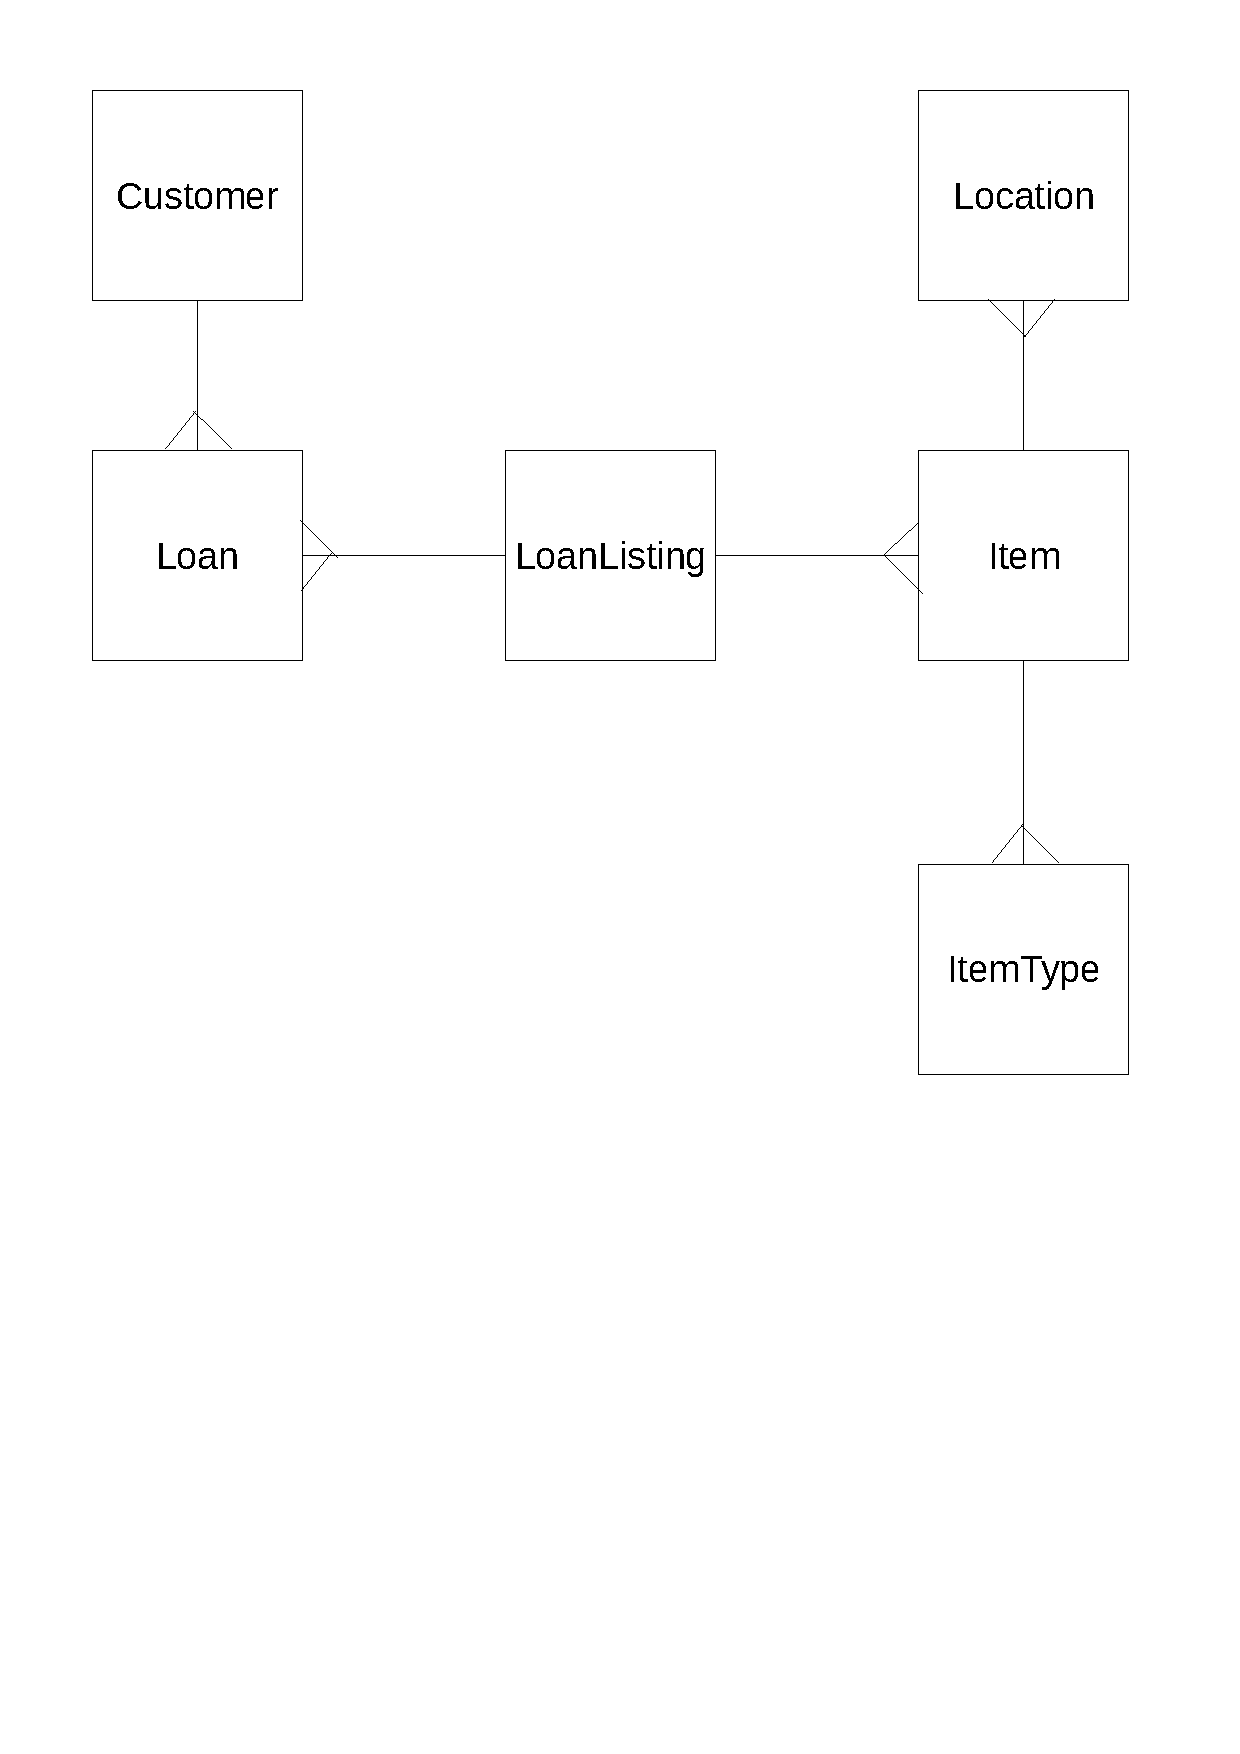
\includegraphics[width=200px]{./Analysis/ER_Diagrams/Loan_ER_Diagrams.pdf}}
    \caption{Loan Item ER Diagrams.} \label{fig:ER Diagrams}
\end{figure}

\begin{figure}[H]
    \centerline{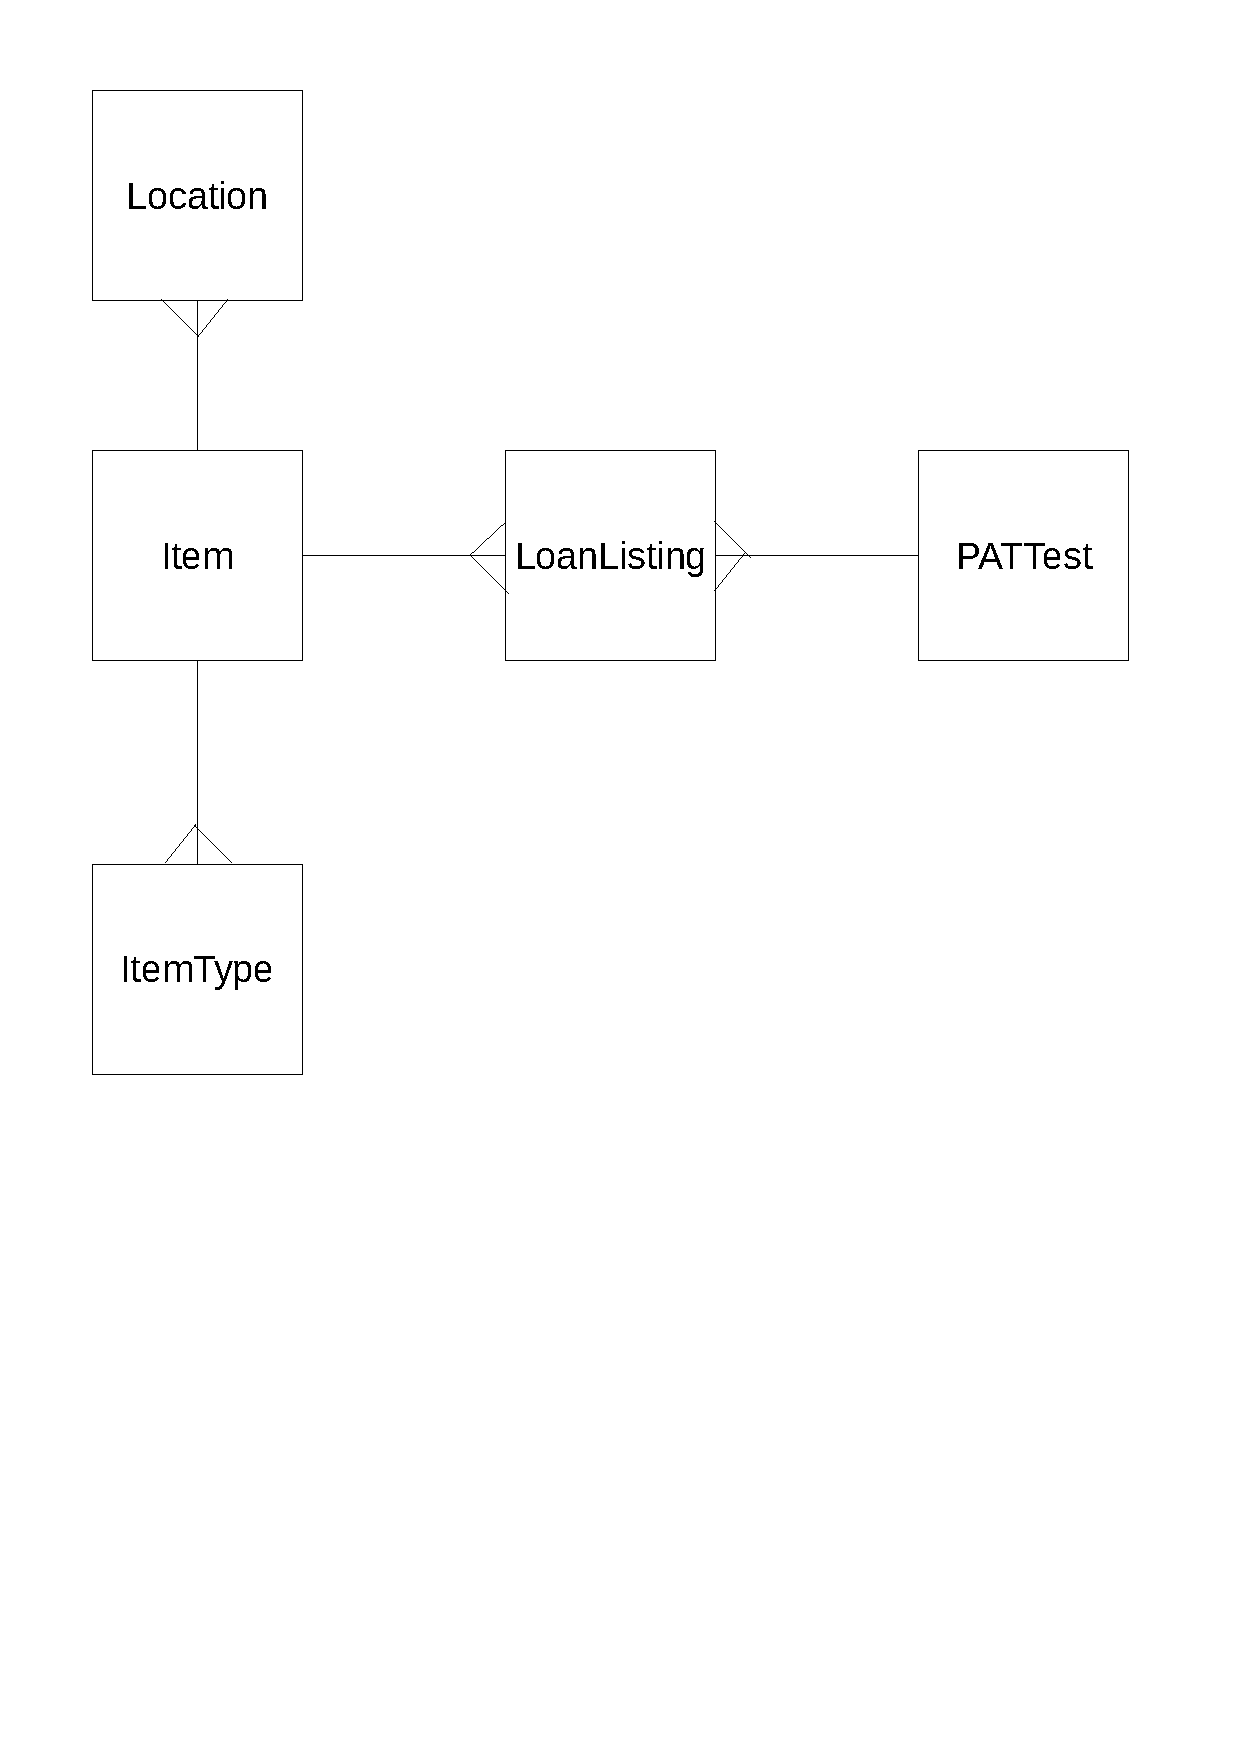
\includegraphics[width=200px]{./Analysis/ER_Diagrams/PAT_Test_ER_Diagrams.pdf}}
    \caption{PAT Test ER Diagrams.} \label{fig:ER Diagrams}
\end{figure}

\subsection{Entity Descriptions}

\noindent \textbf{ItemType}(\underline{ItemTypeID}, ItemType)\\

\noindent \textbf{Location}(\underline{LocationID}, Location)\\

\noindent \textbf{Item}(\underline{ItemID}, \emph{ItemTypeID}, \emph{LocationID}, Name, Location, Value,\\
ItemQuantity, SubTotal, OnLoan,)\\

\noindent \textbf{LoanListing}(\underline{LoanListingID}, \emph{ItemID}, ListingQuantity)\\

\noindent \textbf{Loan}(\underline{LoanID}, \emph{CustomerID}, LoanRate, LoanLength, LoanCost)\\

\noindent \textbf{Customer}(\underline{CustomerID}, Forename, Lastname, Company, Street, Town, County,\\
PostCode, MobileNumber, LandLine, Email)\\

\noindent \textbf{PATtest}(\underline{PATtestID}, TestDate)\\ 

\noindent \textbf{ItemTest}(\underline{ItemTestID}, \emph{PATTestID}, ItemDescription, ItemClass,\\
FuseRating, TestUsed, ProtectiveCondTest, InsulationTest, Leakage, TestResult)\\

\section{Object Analysis}

\subsection{Object Listing}

\begin{itemize}
    \item Client
    \item Item
    \item Location
\end{itemize}

\subsection{Relationship diagrams}

\begin{figure}[H]
    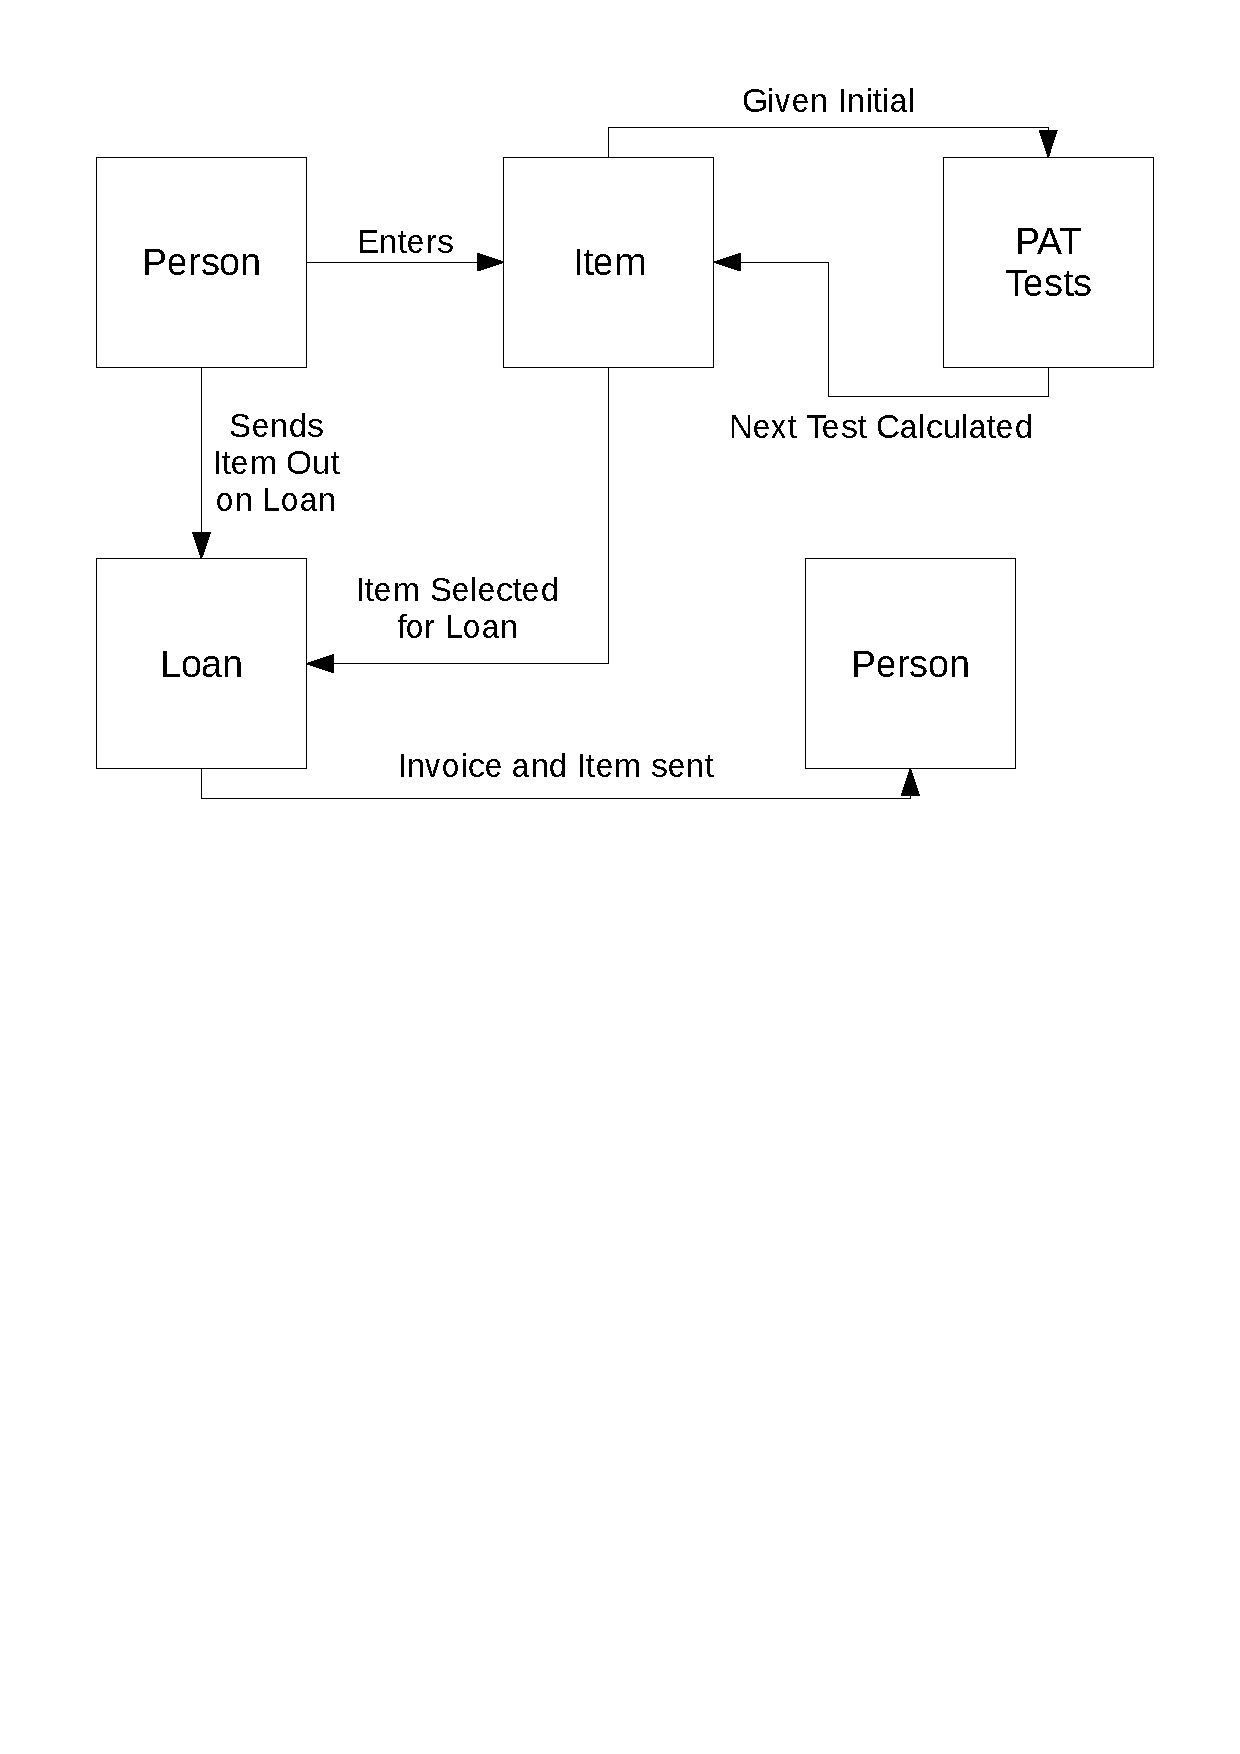
\includegraphics[width=\textwidth]{./Analysis/Relationship_Diagrams/Relationships_diagrams.pdf}
    \caption{Relatioship Diagram.} \label{fig:relationship_diadram}
\end{figure}

\newpage

\begin{landscape}

\subsection{Class definitions}

    \begin{figure}[H]
        \centerline{\includegraphics[width=50px]{./Analysis/Class_Definitions/Class_definition_key.pdf}}
        \caption{Class Diagram Key.} \label{fig:relationship_diagram}
    \end{figure}

    \begin{figure}[H]
        \centerline{\includegraphics[width=450px]{./Analysis/Class_Definitions/Class_diagrams.pdf}}
        \caption{Class Diagrams.} \label{fig:relationship_diagram}
    \end{figure}
\end{landscape}

\newpage

\section{Other Abstractions and Graphs}

\section{Constraints}

\subsection{Hardware}

Presently, Josh uses a custom built, 2008 MacPro Desktop Computer. This is primarily used as a file server for images, audio and video files a well as a backup for his current work desktop. My system will need to be compatible with this system.\\

\noindent Computer Specifications:
\begin{itemize}
    \item 2x 2.8 GHz Quad-Core Intel\textregistered Xeon\texttrademark Processor
    \item ATI Radeon HD 2600 XT 256MB Graphics Card
    \item 661-4449 Apple Mac Pro A1186 Motherboard
    \item 16.00GB DDR3 RAM
    \item 1TB SATA Disk-Drive
    \item 6TB RAID Storage
    \item Apple SuperDrive
    \item 15" LG E1942 LCD Display. 1280 x 720 pixels
\end{itemize}

\noindent The proposed system should have little to no impact on this machine as the processing power and memory that can be dissipated by the computer, greatly exceeds the requirements for the proposed system.\\

\noindent One other constraint of the computer to be used is that it is a desktop computer. This means that the system is only accessible where Josh chooses to have the computer based in his place of work, as the computer is not portable. In addition to this, the computer requires a constant supply of power in order to operate as there is not internal battery.\\

\noindent One other constraint of the computer to be used is that it is a desktop computer. This means that the system is only accessible where Josh chooses to have the computer based in his place of work, as the computer is not portable. In addition to this, the computer requires a constant supply of power in order to opperate as there is not internal battery.\\

\subsection{Software}

Josh has told me that he is able to adapt to the software that is required to run the system. The current operating system in place is Apples OSX 10.8 (Mountain Lion). Josh wishes to update the software sometime in the near future to OSX 10.9 (Mavericks) and possibly update to OSX 10.10 (Yosemite). This could prove to be constraint because OSX 10.10 (Yosemite) isn't yet fully supported by some applications. 

\subsection{Time}

Josh has said that there is no deadline requirement for the proposed system to be in place and doesn't need it until I have finished implementing it. The only deadline I need to meet is the project deadline set by my Computing course leader. This is Friday 13 \textsuperscript{th} February 2014.

\subsection{User Knowledge}

Josh posses a qualification in A level Media studies as well as 2 years use of computers during his degree. He has substantial understanding of how to use computers as his job requires he uses one most of the time. Josh also has required knowledge of how to use many varieties of applications. He uses Adobe Creative Suite for most of his job as he designs various forms of media. He also has knowledge of Apple's Final Cut Pro application as well as many others.\\

\noindent When designing and implementing the proposed system, Josh's experience with computers will have to be considered. Josh tends to use the internet browser Google Chrome for all his web-browsing and research as well as a third party mail application called. By designing the system similarly to these applications, it should make it easier to understand how the system works and get used to using it a lot faster than it would if the system had a primitive design.\\

\noindent There will also be a full manual included to aid Josh with learning and understanding the familiar interface, the functionality of the new system and how to use certain features.

\subsection{Access restrictions}

The proposed system is primarily to be accessed by Josh himself. However, he can see it being an advantage if other people had access to the system.\\

\noindent For this reason, we have agreed that having the database password protected is the best way for Josh to control who can access the data. He will be able to distribute the passwords to other colleagues who he feels should have access to the database management system. This reduces the risk of records being changed or deleted by people who shouldn't need to use the system.

\section{Limitations}

\subsection{Areas which will not be included in computerisation}

Initial buying of new items will not be included in the computerisation as this is still done either in person or over the world wide web. Similarly, initial sales of items will not be included in the computerisation, it will only be once the item has been bought/sold that the data will be updated to coincide with the quantity changes and/or addition to or deduction or equipment.

\subsection{Areas considered for future computerisation}

When a customer loans out equipment, Josh sends out an initial quote, either as an email format or on paper. This could be included in the system by selecting the items the customer wants to high out, and draft a quote form for Josh. Similarly, Josh sends out an emailed invoice to the client, he does this manually by hand. It would be advantageous to include this into the system, by generating an invoice based on the attributes in Loan Records and export it as a PDF for email or printing. These could be implemented in addition to the current database design at the end, if I have enough time to learn and understand how to enter this functionality it into the system

\section{Solutions}

\subsection{Alternative solutions}

\begin{center}
    \begin{tabular}{|p{3cm}|p{6cm}|p{6cm}|}
        \hline
        \textbf{Alternative solution} & \textbf{Advantages} & \textbf{Disadvantages}\\ \hline
        Custom made database & \begin{itemize} \item No need to install additional software, only a simple database management system such as "Microsoft Access" or "Filemaker". \end{itemize} & \begin{itemize} \item Database management systems often cost a substantial amount of money for a license. \end{itemize}\\ \hline
        Web based application & \begin{itemize} \item Easily accessible by other users. Doesn't rely on one machine. \item Can have 'Cloud based' storage of files. \item More than one user can be logged on at a time. \end{itemize} & \begin{itemize} \item Website or server hosting can be expensive. \item More advanced security methods will be required due to the system being constantly online and therefore vulnerable to attack. \item Better networking knowledge required to compensate for the security implications and risks. \end{itemize}\\ \hline
    \end{tabular}
\end{center}

\begin{center}
    \begin{tabular}{|p{3cm}|p{6cm}|p{6cm}|}
        \hline
        \textbf{Alternative solution} & \textbf{Advantages} & \textbf{Disadvantages}\\ \hline            
        Terminal or Command based application & \begin{itemize} \item More power efficient as it isn't graphics heavy, much easier to design as the interface is just text. \item Fast efficient operation provided the client has knowledge of terminal and shell commands. \end{itemize} & \begin{itemize} \item Careful error handling needed as the user could enter any known/valid command. \item Training is required so that the client knows what commands to use when. \item There are often commands that the client don't know about that could potentially corrupt his computer. \end{itemize}\\ \hline
        Python desktop application with a GUI & \begin{itemize} \item Designed and layout can be client specific. \item Minimal error with radio buttons and other widgets. \item Easy to understand layout as data can be formatted to fit the clients requirements. \item Easy to visualise what is happening with graphs and tables. \end{itemize} & \begin{itemize} \item More time needed to build the interface and sql database compared to a command based application. \item More resources needed from the computer for graphical visualisation and database storage \item Programming the graphical interface could prove a difficult task. \end{itemize}\\ \hline
    \end{tabular}
\end{center}


\subsection{Justification of chosen solution}

I have chosen to use the \emph{'Python Desktop Application with a GUI'} solution. \\

\noindent These are my reasons:

\begin{itemize}
    \item The application takes up no physical space apart from the computer it is installed on.
    \item I already have the required language knowledge needed to program a database and a GUI in Python
    \item Using a custom made desktop application is faster for Josh to manage his inventory than the current spreadsheet based system.
    \item Backup can be made and data can be restored easily in the event of corruption or unresolvable data loss
\end{itemize}
